%\documentclass{cumcmthesis}
\documentclass[withoutpreface,bwprint]{cumcmthesis} %去掉封面与编号页

\title{基于状态空间方程的波浪能装置最大功率优化设计}
\tihao{A}            % 题号
\baominghao{4321}    % 报名号
\schoolname{你的大学}
\membera{成员A}
\memberb{成员B}
\memberc{成员C}
\supervisor{指导老师}
\yearinput{2017}     % 年
\monthinput{08}      % 月
\dayinput{22}        % 日

\begin{document}
    \maketitle
    \begin{abstract}
        波浪能是一种重要的可再生能源,具有可观的应用前景。使用以浮子与振子及之间的阻尼装置为核心的波浪能装置是常见的利用波浪能的方法。
        其中,阻尼装置的相关参数(如阻尼系数)对波浪能的利用率有显著影响。
        本文基于\textbf{力学分析}方法,通过\textbf{局部线性化方法}构建了波浪能装置的\textbf{状态空间方程},建立起波浪能装置中浮子、振子的运动模型,求解了波浪能装置中浮子和振子在一段时间内的(角)位移与速度的变化情况,
        并以此为基础,通过\textbf{搜索法}和\textbf{遗传算法}对阻尼器参数进行优化,进而求出装置的最大输出功率及相应的最优阻尼系数。
        
        \textbf{针对问题一},浮子和振子只做垂荡运动,本文通过将波浪能装置的运动抽象为\textbf{二自由度的弹簧阻尼模型},
        结合\textbf{牛顿第二定律},通过构造状态向量并建立状态空间方程,将多条力学定律约束转换为一阶线性非齐次矩阵微分方程,
        然后使用$Picard$定律证明解的存在性与唯一性,
        并基于常微分方程知识与数值积分方法分别给出解析解与数值解。
        对于第二小问,对非线性的阻尼力进行\textbf{局部线性化},建立局部状态空间方程,用\textbf{迭代法}不断在每一时间步上求解局部状态空间方程,
        给出离散时间步上的数值解。
        最终得到浮子和振子在前$40$个周期内时间间隔为$0.2s$的垂荡位移和速度。结果详细见\cref{tab:1.1}与\cref{tab:1.2} 。
    
        \textbf{针对问题二},由垂荡运动模型推导出平均输出功率的积分形式,并使用梯形法进行数值积分。
        且由于开始部分受初值选取影响较大,故选用装置状态已经稳定时(后二十秒)的数据进行计算。
        由于第一问只需优化直线阻尼系数一个变量,为\textbf{单变量优化模型},故采用\textbf{搜索法},求得最大平均输出功率为$229.997w$,最优直线阻尼系数为$37993$;
        第二问为需要优化的变量有两个,为\textbf{多变量优化模型},故先用搜索法缩小范围,再采用\textbf{遗传算法}获得较好的解,求得最大平均输出功率为$230.402w$,最优直线阻尼系数为$37779$, 幂指数为$0.0001$。
    
        \textbf{针对问题三},浮子和振子不仅做垂荡运动,而且做固定平面内的纵摇运动。首先,通过\textbf{平行轴定理}得到浮子相对质心轴的转动惯量,
        并给出振子相对于旋转阻尼器轴的转动惯量表达式。
        然后,采用和问题一类似的方法分别列出装置垂荡和纵摇状态下的状态空间方程, 并将其转化成\textbf{局部线性的状态空间方程}。
        最后求得装置在前$40$个周期内间隔$0.2s$的垂荡位移和速度、角位移和角速度。结果详细见\cref{tab:3.1}与\cref{tab:3.2}。
    
        \textbf{针对问题四},由纵摇运动模型推导出旋转阻尼器平均输出功率表达式, 并使用梯形法进行数值积分,
        同样选取后20秒的稳定区域进行计算。然后同时考虑两种阻尼器的平均输出功率,建立以二者之和最大为目标的\textbf{单目标优化模型},
        由于优化的变量有两个,同样使用先搜索后使用遗传算法的优化方法,求得最大平均输出功率为$316.518w$,最优直线阻尼系数为$60448$, 最优旋转阻尼系数为$100000$。
            \keywords{二自由度的弹簧阻尼模型\quad  局部线性化\quad 状态空间方程\quad  矩阵微分方程\quad 遗传算法}
    \end{abstract}
    % \tableofcontents % 目录
    \section{问题重述}
    \subsection{问题的背景}
    在过去的几十年里,经济和社会飞速发展,能源问题、污染问题日益严重,发展清洁的可再生能源已成为世界各国的共识。
    海洋蕴含着巨大的能量,如波浪,潮汐,洋流,近海风,海洋热能等,其中海上风力发电技术已进入商业化应用阶段。
    此外,波浪能作为一种易获得的可再生能源,因其分布广泛、储量丰富,也具有不错的商业化前景。
    研究如何提升波浪能装置的能量转换效率是波浪能规模化利用的一个关键性问题。
    \subsection{问题的重述}
    有一种波浪能装置由浮子、振子、弹簧、阻尼器组成。在波浪的作用下,浮子带动振子运动,从而驱动阻尼器做功,所做功作为能量输出。
    
    基于以上装置,需要建立数学模型解决以下问题:

    \textbf{问题一}:考虑浮子在波浪激励力为$f\cos\omega t$ 的作用下只做垂荡运动。
    分别计算在两种情况下,浮子与振子在前$40$个波浪周期内,时间间隔为$0.2s$的垂荡位移与速度。
    情况一中,直线阻尼器的阻尼系数为$10000N\cdot s/m$;
    情况二中,直线阻尼器的阻尼系数与浮子和振子相对运动的绝对值的$0.5$次幂成正比,比例系数为 $10000$。

    \textbf{问题二}:在问题一的基础上,考虑浮子在波浪中只做垂荡运动,
    分别计算两种情况的最大输出功率及相应的最优阻尼系数。
    情况一中,直线阻尼器的阻尼系数为常数,在$[0, 100000]$内取值;
    情况二中,直线阻尼器的阻尼系数与浮子和振子相对运动的绝对值的幂成正比,比例系数在$[0, 100000]$中取值,幂指数在$[0, 1]$中取值。

    \textbf{问题三}:除直线阻尼器外,还安装旋转阻尼器和扭转弹簧,装置由直线阻尼器和旋转阻尼器共同提供输出。
    浮子在波浪激励力为$f\cos\omega t$,波浪激励力矩为$L\cos\omega t$ 的作用下做垂荡和纵摇运动。
    在直线阻尼器的阻尼系数为$10000$,旋转阻尼器的阻尼系数为$1000$的情况下,
    求浮子与振子在前$40$个波浪周期内,时间间隔为$0.2s$的垂荡位移与速度、纵摇角位移与角速度。

    \textbf{问题四}:在问题三的基础上,考虑浮子只做垂荡和纵摇运动,
    分别计算装置的最大输出功率及相应最优阻尼系数
    直线阻尼器阻尼系数为常数,在$[0, 100000]$取值,
    旋转阻尼器阻尼系数均为常数,在$[0, 100000]$取值。
    \section{问题分析}
    \subsection{问题一的分析}
    问题一中考虑只装置在垂荡方向的运动。对浮子振子两个物体分别进行受力分析,通过牛顿第二定律列出两个物体的运动方程。

    第一小问:直线阻尼器的阻尼系数为常数,则方程中涉及的所有力(最终反馈为浮子、振子的加速度)
    要么可以用浮子、振子的位置与速度的线性组合表示,要么仅与时间相关。
    因此,可将浮子的位置、速度,振子的位置、速度写为一个状态向量,状态向量关于时间的导数可表达为状态向量与某一矩阵的乘积
    (对应第一类力)与仅与时间相关的输入向量的和(对应第二种力),从而建立一阶线性矩阵微分方程。
    
    第二小问:直线阻尼器的阻尼系数和振子浮子的速度差的$0.5$次幂成正比,阻尼力无法写为浮子、振子的位置与速度的线性组合,
    故不能将装置纵摇运动的状态空间方程直接转换为线性矩阵微分方程。因此,考虑使用一阶泰勒展开对阻尼力进行局部线性化,从而在局部建立起
    线性矩阵微分方程,然后进行迭代:不断求解局部方程、获取下一时间步的状态向量、更新方程初始值,直到获得所有时间步上的状态向量。
    \subsection{问题二的分析}
    问题二要求在问题一的基础上,求出最优的阻尼系数来实现装置的最大平均功率,

    第一小问规定直线阻尼器的阻尼系数取值范围为$[0,100000]$,需要求出直线阻尼器有最大平均功率时的阻尼系数。
    由于问题为单目标单变量优化问题,故采用暴力搜索法求得最优阻尼系数。
    由功率的计算公式$P=F\cdot v$ 求出直线阻尼器的平均功率表达式。
    因速度数据为离散形式,故采用梯形面积的累加来代替积分面积的计算。
    由于刚开始运动时装置未达到稳态,数据波动较大,故采用最后$20$秒的稳定状态的数据进行计算。

    第二小问规定比例系数为$[0,100000]$,幂指数的范围为$[0,1]$,
    功率的计算同第一小问。
    由于问题为多变量优化问题,
    故应先搜索缩小参数范围,再通过遗传算法求出最优参数。

    \subsection{问题三的分析}
    问题三在垂荡的基础上,还要考虑装置的纵摇运动,同时引入扭转弹簧和旋转阻尼器。
    通过刚体的定轴转动定律列出两个物体纵摇的动力方程,再将其转化为状态空间方程。
    将装置垂荡和纵摇的状态空间方程分别求解,得到最终数值解。
    \subsection{问题四的分析}
    问题四要求在问题三的基础上,求出最优的阻尼系数来实现装置的最大平均功率。
    规定了直线阻尼器的阻尼系数范围为$[0,100000]$,旋转阻尼器的阻尼系数范围为$[0,100000]$。
    针对旋转阻尼器的平均功率,使用$P = M\cdot \beta$求出其表达式。
    采用和问题二相同的方法离散化处理积分面积,并采用最后$20$秒的稳定状态进行计算,
    问题转化为目标为二者功率之和的单目标优化问题。
    由于问题为多变量优化问题,故应先搜索缩小参数范围,再通过遗传算法求出最优参数。

    \section{模型假设}
    \begin{enumerate}
        \item 忽略中轴、底座、隔层、PTO的质量和各种摩擦。
        \item 假设海水无粘及无旋。
        \item 忽略装置除波浪激励力,附加惯性力,兴波阻尼力、静水恢复力,重力,浮力之外所受的一切外力。
        \item 假设初始时装置在静水中静止。
        \item 假设振子和浮子的质量分布均匀。
        \item 假设水面仅在浮子圆柱部分浮动。 
        \item 忽略纵摇运动对垂荡运动的影响。 
    \end{enumerate}
    \section{符号说明}
    \begin{longtable}{ccc}
        \label{tab:symbol} \\
        \toprule[1.5pt]
        \makebox[0.3\textwidth][c]{符号} & \makebox[0.3\textwidth][c]{意义} & \makebox[0.3\textwidth][c]{单位} \\
        \midrule[0.75pt]
        \endfirsthead
        \toprule[1.5pt]
        \endhead
        \bottomrule[1.5pt]
        \endfoot
        $m_1$ & 浮子质量 & $kg$ \\
        $m_2$ & 振子质量 & $kg$ \\
        $m_3$ & 垂荡附加质量 & $kg$ \\
        $J_1$ & 浮子转动惯量 & $kg\cdot m^2$ \\
        $J_2$ & 振子转动惯量 & $kg\cdot m^2$ \\
        $J_3$ & 纵摇附加转动惯量 & $kg\cdot m^2$ \\
        $r_1$ & 浮子底半径 & $m$ \\
        $r_2$ & 振子半径 & $m$ \\
        $h_{1y}$ & 浮子圆柱部分高度 & $m$ \\
        $h_{1z}$ & 浮子圆锥部分高度 & $m$ \\
        $h_2$ & 振子高度 & $m$ \\
        $x_1$ & 浮子隔层位移 & $m$ \\
        $x_2$ & 振子底部位移 & $m$ \\
        $\theta_1$ & 浮子角位移 & $rad$ \\
        $\theta_2$ & 振子角位移 & $rad$ \\
        $\rho$ & 海水的密度 & $kg/m^3$ \\
        $g$ & 重力加速度 & $m/s^2$ \\
        $k$ & 直线弹簧刚度 & $N/m$ \\
        $K$ & 扭转弹簧刚度 & $N\cdot m$ \\
        $b$ & 直线阻尼系数 & $N\cdot s/m$ \\
        $B$ & 旋转阻尼系数 & $N\cdot m\cdot s$ \\
        $b_1$ & 垂荡兴波阻尼系数 & $N\cdot s/m$ \\
        $B_1$ & 纵摇兴波阻尼系数 & $N\cdot m\cdot s$ \\
        $f$ & 垂荡激励力振幅 & $N$ \\
        $L$ & 纵摇激励力矩振幅 & $N\cdot m$ \\
        $\omega$ & 入射波浪频率 & $s^{-1}$ \\
    \end{longtable}  
    \section{模型的建立与求解}
    \subsection{问题一模型的建立与求解}
    \subsubsection{模型的建立}
    问题一只考虑装置在竖直方向的运动,具体由可分为浮子在竖直方向的一维运动与振子在竖直方向上
    的一维运动,故整个系统的自由度为$2$,整个系统的状态可以被浮子在竖直方向的位置、浮子在竖直方向的速度、
    振子在竖直方向上的位置、振子在竖直方向上的速度四个量完全确定。故本文定义如下向量作为系统的状态向量:
    $$
    z = \left [
        \begin{array}{c}
        x_1 \\
        v_1 \\
        x_2 \\            
        v_2 \\
        \end{array} \right ]
    $$
    其中,$ x_1 $表示浮子在竖直方向的位置,即浮子圆锥部分与圆柱部分的交界面到海平面的有向距离,
    $ v_1 $表示浮子在竖直方向的速度,
    $ x_2 $表示振子在竖直方向的位置,即振子下端到海平面的有向距离,
    $ v_2 $表示振子在竖直方向的速度。状态变量中的所有分量均以竖直向上为正方向。

    \begin{figure}[H]
        \centering
        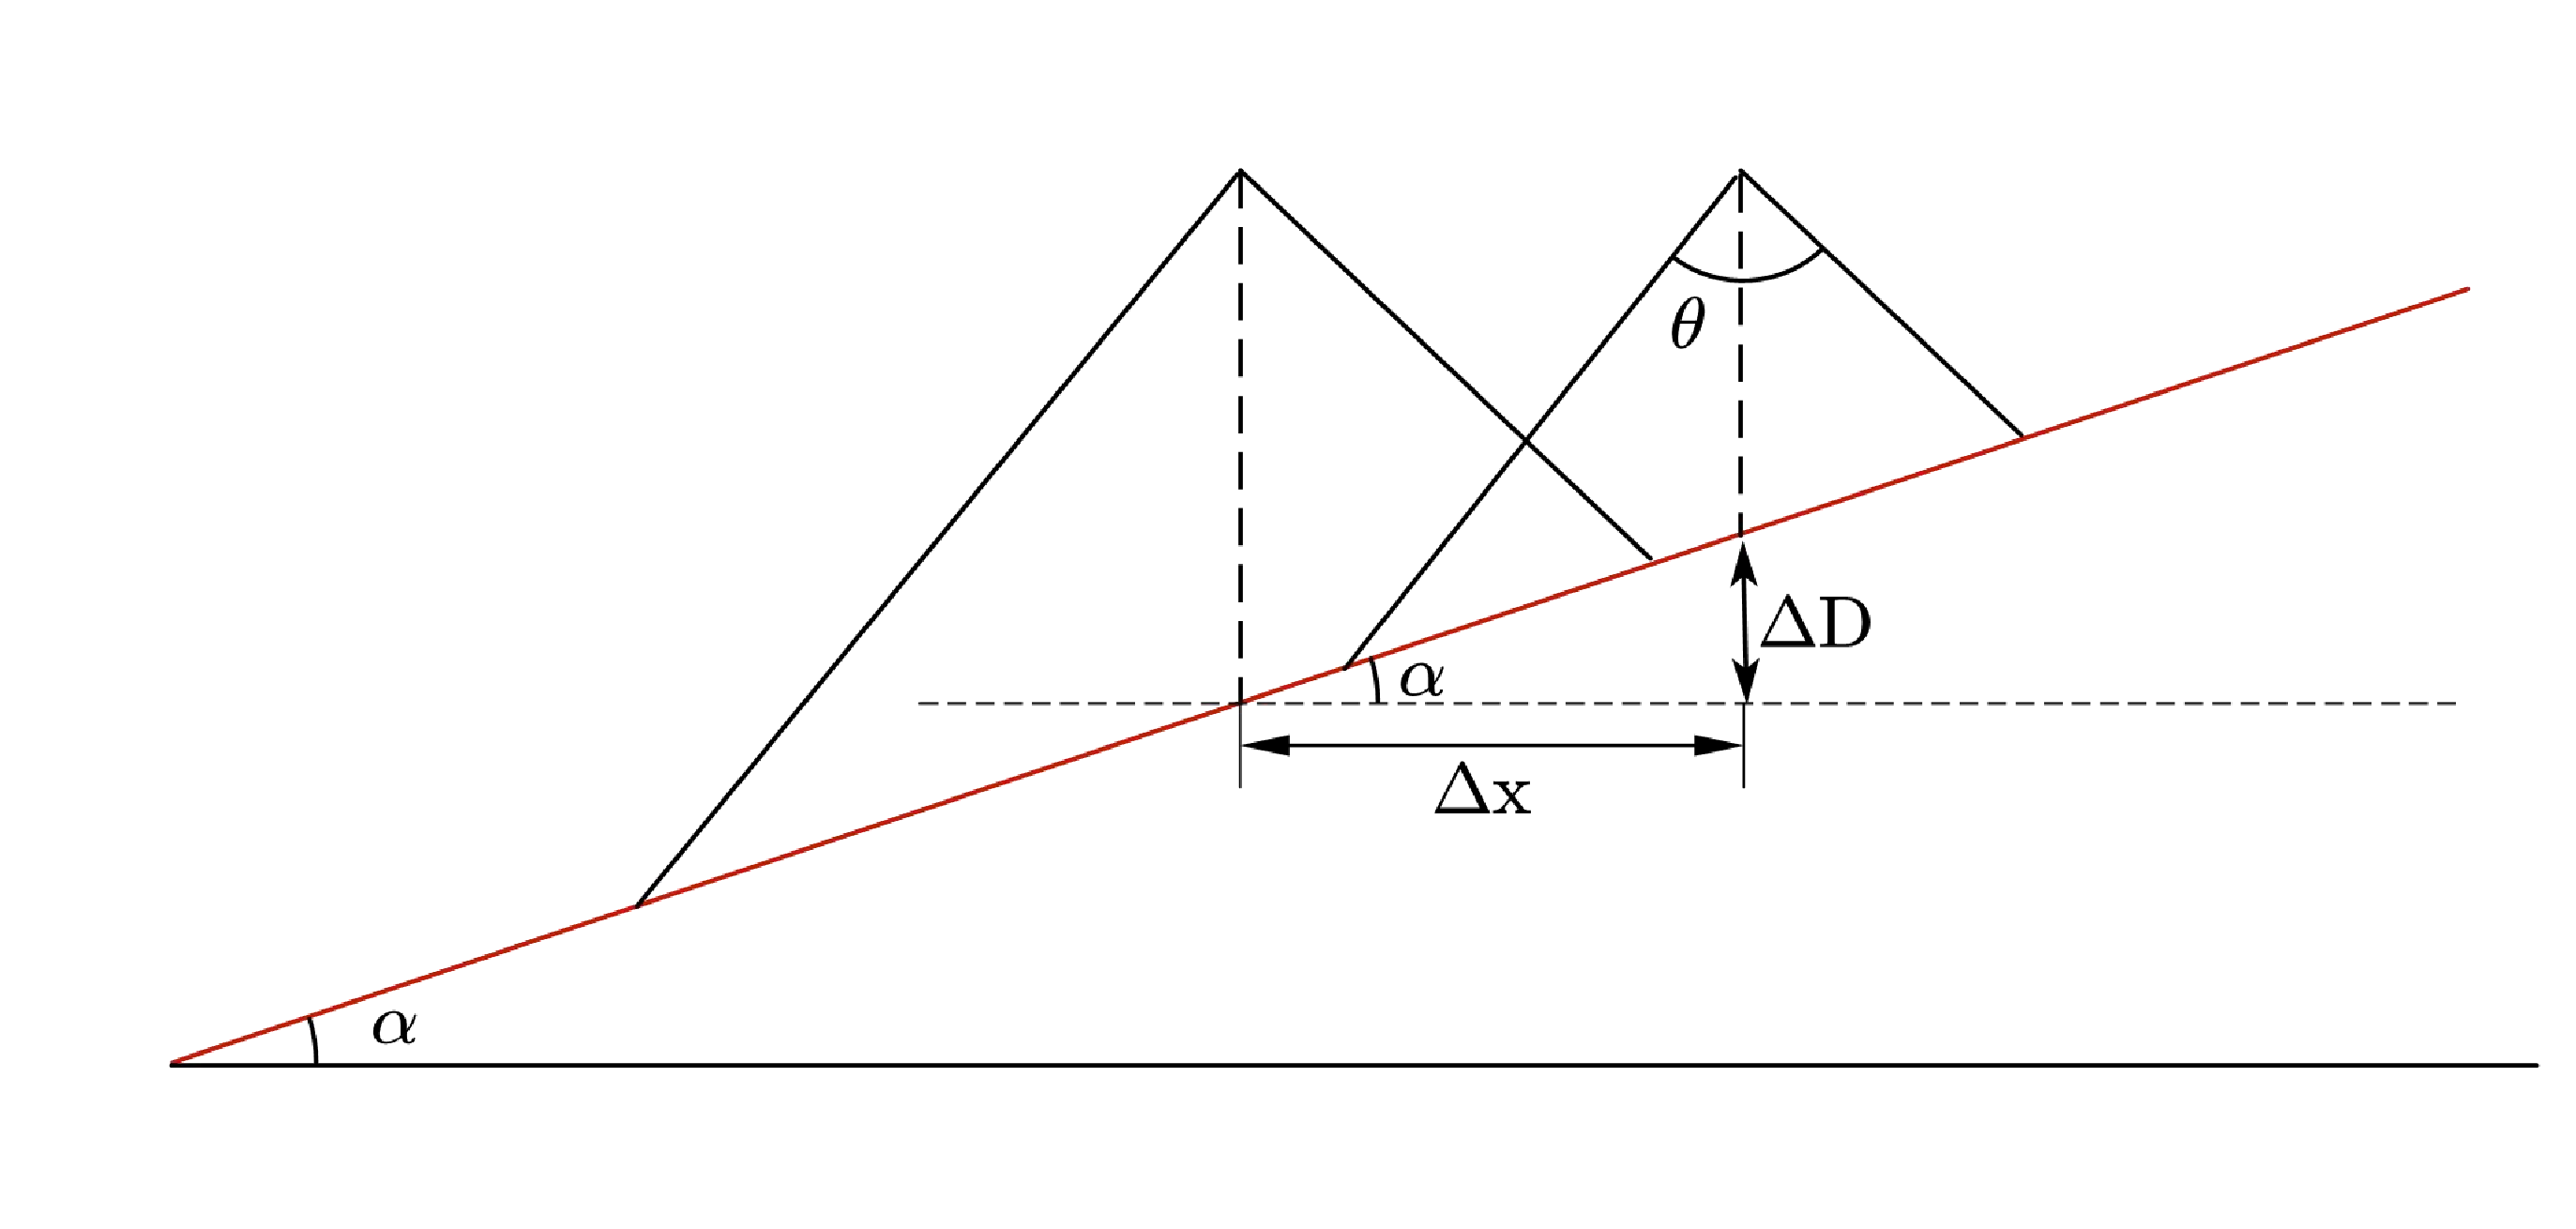
\includegraphics[width=.7\textwidth, height=5cm]{f1}
        \caption{浮子坐标示意图}
        \label{fig:coordinate}
    \end{figure}
    
    现先仅考虑直线阻尼器阻尼系数为常数的情况,
    对系统进行受力分析:\\
    \textbf{浮子所受波浪激励力}: 
    \begin{equation}
        F_w = f \cos\omega t 
        \label{eq:wave}
    \end{equation}
    \textbf{浮子所受浮力或静水恢复力}:
    \begin{equation}
        F_b = \rho g V 
        \label{eq:buoyancy}
    \end{equation}其中 $V$ 为浮子在海平面下的体积。
    \textbf{浮子重力}:
    \begin{equation}
        G_1 = m_1 g
        \label{eq:G1}
    \end{equation} 其中 $m_1$ 为浮子的质量。
    \textbf{振子重力}:
    \begin{equation}
        G_2 = m_2 g
        \label{eq:G2}
    \end{equation} 其中 $m_2$ 为浮子的质量。
    \textbf{兴波阻尼力}: 
    \begin{equation}
        F_{d1} = b_1\dot{x_1}
        \label{eq:d1}
    \end{equation} 其中$b_1$为垂荡兴波阻尼系数。
    \textbf{直线弹簧弹力}: 
    \begin{equation}
        F_e = k(x_0 - (x_2 - x_1))
        \label{eq:e}
    \end{equation} 其中$k$为直线弹簧刚度,$x_0$ 为弹簧原长。
    \textbf{直线阻尼器阻尼力}:
    \begin{equation}
        F_d = b(\dot{x_1} - \dot{x_2})
        \label{eq:d}
    \end{equation} 其中$b$为直线阻尼系数。
    根据\textbf{牛顿第二定律}可列方程如下:
    \begin{equation}
        \begin{cases}
            G_1 + F_w + F_b + F_{d1} - F_e - F_d = (m_1 + m_3) \ddot{x_1}\\
            G_2 + F_e + F_d = m_2 \ddot{x_2}
        \end{cases}
        \label{eq:newton}
    \end{equation}
    其中 $m_3$ 为垂荡附加质量。

    本文将以上力拆分为两类:1.恒力或只与时间相关的力,2.与状态向量的分量呈线性关系的力。
    依据此标准,可将\textbf{浮子浮力}拆为两部分:
    \begin{equation}
        F_b = \rho g V_0 + \rho g \pi r_1^2 x_1
        \label{eq:split_b}
    \end{equation} 其中$V_0 = 1/3 \pi r_1^2 h_{1z}$为浮子圆锥部分的体积,$r_1$ 为浮子底半径。
    同理,可将\textbf{直线弹簧的弹力}拆分为两部分: 
    \begin{equation}
        F_e = k x_0 - k(x_2 - x_1)
        \label{eq:split_e}
    \end{equation} 对系统中的力进行拆解后,本文中将第一类力作为系统的外部输入,将第二类力以动力方程的形式表达,最终建立状态空间方程如下:
    \begin{equation}
        \dot{z}= Az + Bu
        \label{eq:space}
    \end{equation}
    其中 $
        A = \left [
        \begin{array}{cccc}
            0 & 1 & 0 & 0 \\
            \frac{-k -\rho g \pi r_1^2}{m_1 + m_3} & \frac{- b - b_1}{m_1 + m_3} & \frac{k}{m_1 + m_3} & \frac{b}{k1 + k3}\\
            0 & 0 & 0 & 1 \\
            \frac{k}{m_2}& \frac{b}{m_2} & \frac{-k}{m_2} & \frac{-b}{m_2}\\
        \end{array} \right ]
        $,
        $
        B = \left [
        \begin{array}{cc}
        0&0\\
        \frac{1}{m_1 + m_3}&0\\
        0&0\\
        0&\frac{1}{m_2}\\
        \end{array} \right ]
        $ \\
        $
        u = \left [
        \begin{array}{c}
        f\cos \omega t - m_1 g + \rho g V_0 - k x_0\\
        -m_2 g + k x_0 \\
        \end{array} \right ]
        $ \\
    上式是一个一阶线性非齐次矩阵微分方程,可以类比一阶线性非齐次微分方程的解法得到通解。
    同时,状态向量的初值$ z_0 $可通过计算确定,故原问题可转化矩阵常微分方程的初值问题求解。
    本文将在模型求解中具体讨论初值的计算、解的存在性,并给出初值条件下的解析解与数值计算结果。

    接下来讨论直线阻尼器的阻尼系数与振子、浮子的相对速度的幂次呈正比的情况。\\
    除直线阻尼器的阻尼力外,其他力的计算方式与第一种情况一致,故不再讨论。

    在题目给定的幂次$(0.5)$下,\textbf{直线阻尼器阻尼力}为:
    \begin{equation}
        F_d = b_0 \sqrt{|v|}v
        \label{eq:d_1}
    \end{equation} 其中 $b_0$ 为比例系数, $v = v_1 - v_2$, $v_1$ 为浮子的垂荡速度,$v_2$ 为振子的垂荡速度。

    阻尼力无法直接以振子、浮子速度的线性组合表达。考虑到线性微分方程具有易证明解的存在性、
    可以给出解析解、适配的数值方法有较高稳定性等优点,本文将阻尼力进行局部的线性化。

    当$v$在$v_0$附近变化时,可以用$F_d(v)$在$v=v_0$处的切线来拟合$F_d$,
    这等价于在$v = v_0(v_0 \neq 0)$ 处对$F_d(v)$做一阶泰勒展开,
    得$ F_d = 1.5 b_0 \sqrt{|v_0|}v - 0.5 b_0\sqrt{|v_0|}v_0$
    该式可将误差控制在$O(h),h = v - v_0 $。

    则原状态空间方程,$ \dot{z}= Az + Bu$ 中的$ A $和$ u $在$ v = v_0 $附近分别变为:

    $$
    A = \left [
        \begin{array}{cccc}
            0&1&0&0 \\
            \frac{-k -\rho g \pi r_1^2}{m_1 + m_3} & \frac{-b - b_1}{m_1 + m_3}
            & \frac{k}{m_1 + m_3} & \frac{b}{k1 + k3}\\
            0&0&0&1 \\
            \frac{k}{m_2}& \frac{b}{m_2} & \frac{-k}{m_2} & \frac{-b}{m_2}\\
        \end{array} \right ]
    $$
    其中,直线阻尼系数$b = 1.5 b_0 |v|^{0.5}$,
    $$
    u = \left [
        \begin{array}{c}
            f\cos \omega t - m_1 g + \rho g V_0 - k x_0 -  0.5 b_0\sqrt{|v_0|}v_0\\
            -m_2 g + k x_0 + 0.5 b_0\sqrt{|v_0|}v_0 \\
        \end{array} \right ]
    $$

    为保证线性化不带来过多精度损失,本文选取一个较小的步长$ \Delta t = 0.01s$, 从初值开始求解状态空间方程,
    计算下一时间步的解,根据解得的状态向量更新$ A, u $,然后将当前解作为新的初值继续求解状态空间方程,
    以此类推可得到目标时间范围内的所有系统状态。更具体的做法将在模型求解中继续讨论。
    \subsubsection{模型的求解}
    求解模型前,本文选取振子、浮子均在水中静止的稳态作为初始状态,并根据平衡条件计算振子、浮子的初始位置。
    已知
    \begin{equation}
        F_b = G_1 + G_2 
        \label{eq:balance_1}
    \end{equation}
    \begin{equation}
        F_e = G_2
        \label{eq:balance_2}
    \end{equation}
    计算可得,模型初始状态为:
    $$
    z_0 = \left [
        \begin{array}{c}
        -2.0 \\
        0 \\
        -1.8 \\            
        0 \\
        \end{array} \right ]
    $$

    现先仅考虑直线阻尼器阻尼系数为常数的情况,设$ f(t, z) = Az + Bu(t) $,
    求解$ \dot{z}= f(z, t) $, $ z_0 = [-2.0, 0, -1.8, 0]$的初值问题。
    取$L$为$A$的特征值绝对值的最大值, 
    显然有$ |f(t, z_1) - f(t, z_2)| \leq L|z_1 - z_2| $,即$ f(t, z) $ 满足$Lipschitz$条件。
    由$ Picard $定理可知该初值问题的解存在且唯一。

    类比一阶线性非齐次常微分方程的解法,可解得状态空间方程的通解为:$$z = e^{tA}(C + \int e^{-tA}Bu(t)dt) $$
    其中矩阵积分定义为对矩阵的元素分别做积分,$ C $为任意四维列向量,$ e^{tA}C $是方程$ \dot{x} = Ax, x_0 = C$的解,
    可展开为$ e^{tA} = I + tA + \frac{1}{2!}t^2A^2 + \frac{1}{3!}t^3A^3 + \cdots $,$ I $为与A同形的单位矩阵。
    上式提供了任意逼近$ e^{tA} $的一个方法。
    已知$ t_0 = 0, z_0 = [-2.0, 0, -1.8, 0]$, 可以给出方程的一个特解:$$ z(t) = e^{tA}z_0 + e^{tA}\int_{t_0}^t e^{-tA}Bu(t)dt $$
    为给出最终的数值解,本文考虑三种方法:

    1. 在较高的阶数截断,如用$ I + tA + \frac{1}{2!}t^2A^2 + \frac{1}{3!}t^3A^3 + \cdots + \frac{1}{7!}t^7A^7 $
    来给出$ e^{tA} $的近似,显然$ z $中的每一元素均为$ \sum\limits_{i=0}^{n}a_it^i\cos\omega t $的形式,$ n $为截断的阶数,则$ z $的
    每一元素均有原函数,故可较方便的给出每一元素的变上限积分的表达式,从而可以直接给出$ z(t) $的表达式,再给出$ z(t) $在时域上
    采样的离散值。考虑到在不同阶数下$ z(t) $的表达式可能有较大差异,且在$ n $较大时逐项求原函数较为麻烦,本文仅证明了该方法的可行性
    并给出了求任意阶截断下的表达式的流程,没有给出具体的可供运算的$ z(t) $的表达式。

    2. 沿用方法一的截断方法,但不求解$ z(t) $的具体表达式,直接用数值积分(梯形法)计算$ e^{tA}\int_{t_0}^t e^{-tA}Bu(t)dt $,
    即将原式离散化为:
    $$ z(t) = e^{tA}z_0
     + e^{tA}\sum\limits_{s = 0}^{\frac{t}{\Delta t}} \frac{1}{2}(e^{-(s \Delta t)A}Bu(s \Delta t) 
     + e^{((s + 1) \Delta t)A}Bu((s + 1)\Delta t))\Delta t $$
    其中$ s $为步数,$ \Delta t $为时间步长,其中$ e^{tA} $可按需取为任意阶截断。
    方法二的优点为较为方便,无需求解原函数,在步长较小时精度较好,缺点为同时引入了$e^tA$截断误差与数值积分时进行离散近似带来的误差,
    难以进行误差分析。

    3. 仅用解析解表达式验证解的性质,直接使用四阶龙格库塔法求解状态空间方程$ \dot{z}= Az + Bu$来给出数值解。
    鉴于该方法已较为成熟,已被广泛使用并集成为各类数值求解工具中求解矩阵微分方程的默认方法,本文不再详述。

    接下来考虑直线阻尼器的阻尼系数与振子、浮子的相对速度的幂次$(0.5)$呈正比的情况。在模型建立中已给出了对直线阻尼器的阻尼力进行局部线性化
    后的局部状态空间方程。本文选取时间步长为$ \Delta t = 0.01s$(应当略大于数值积分时所用的时间步长),
    先求解$ t_0 = 0, z_0 = [-2.0, 0, -1.8, 0]$时的解$z_1(t)$,
    得到$ z_1 = z_1(t_0 + \Delta t) $,
    然后求解$ t_0 \leftarrow t_0 + \Delta t, z_0 \leftarrow z_1$下的解时$z_2(t)$,得到$ z_2 = z_2(t_0 + \Delta t) $,
    以此类推可得到目标时间范围内的$ z_i $ 算法流程图可总结如 \cref{fig:algorithm}:

    \begin{figure}[H]
        \centering
        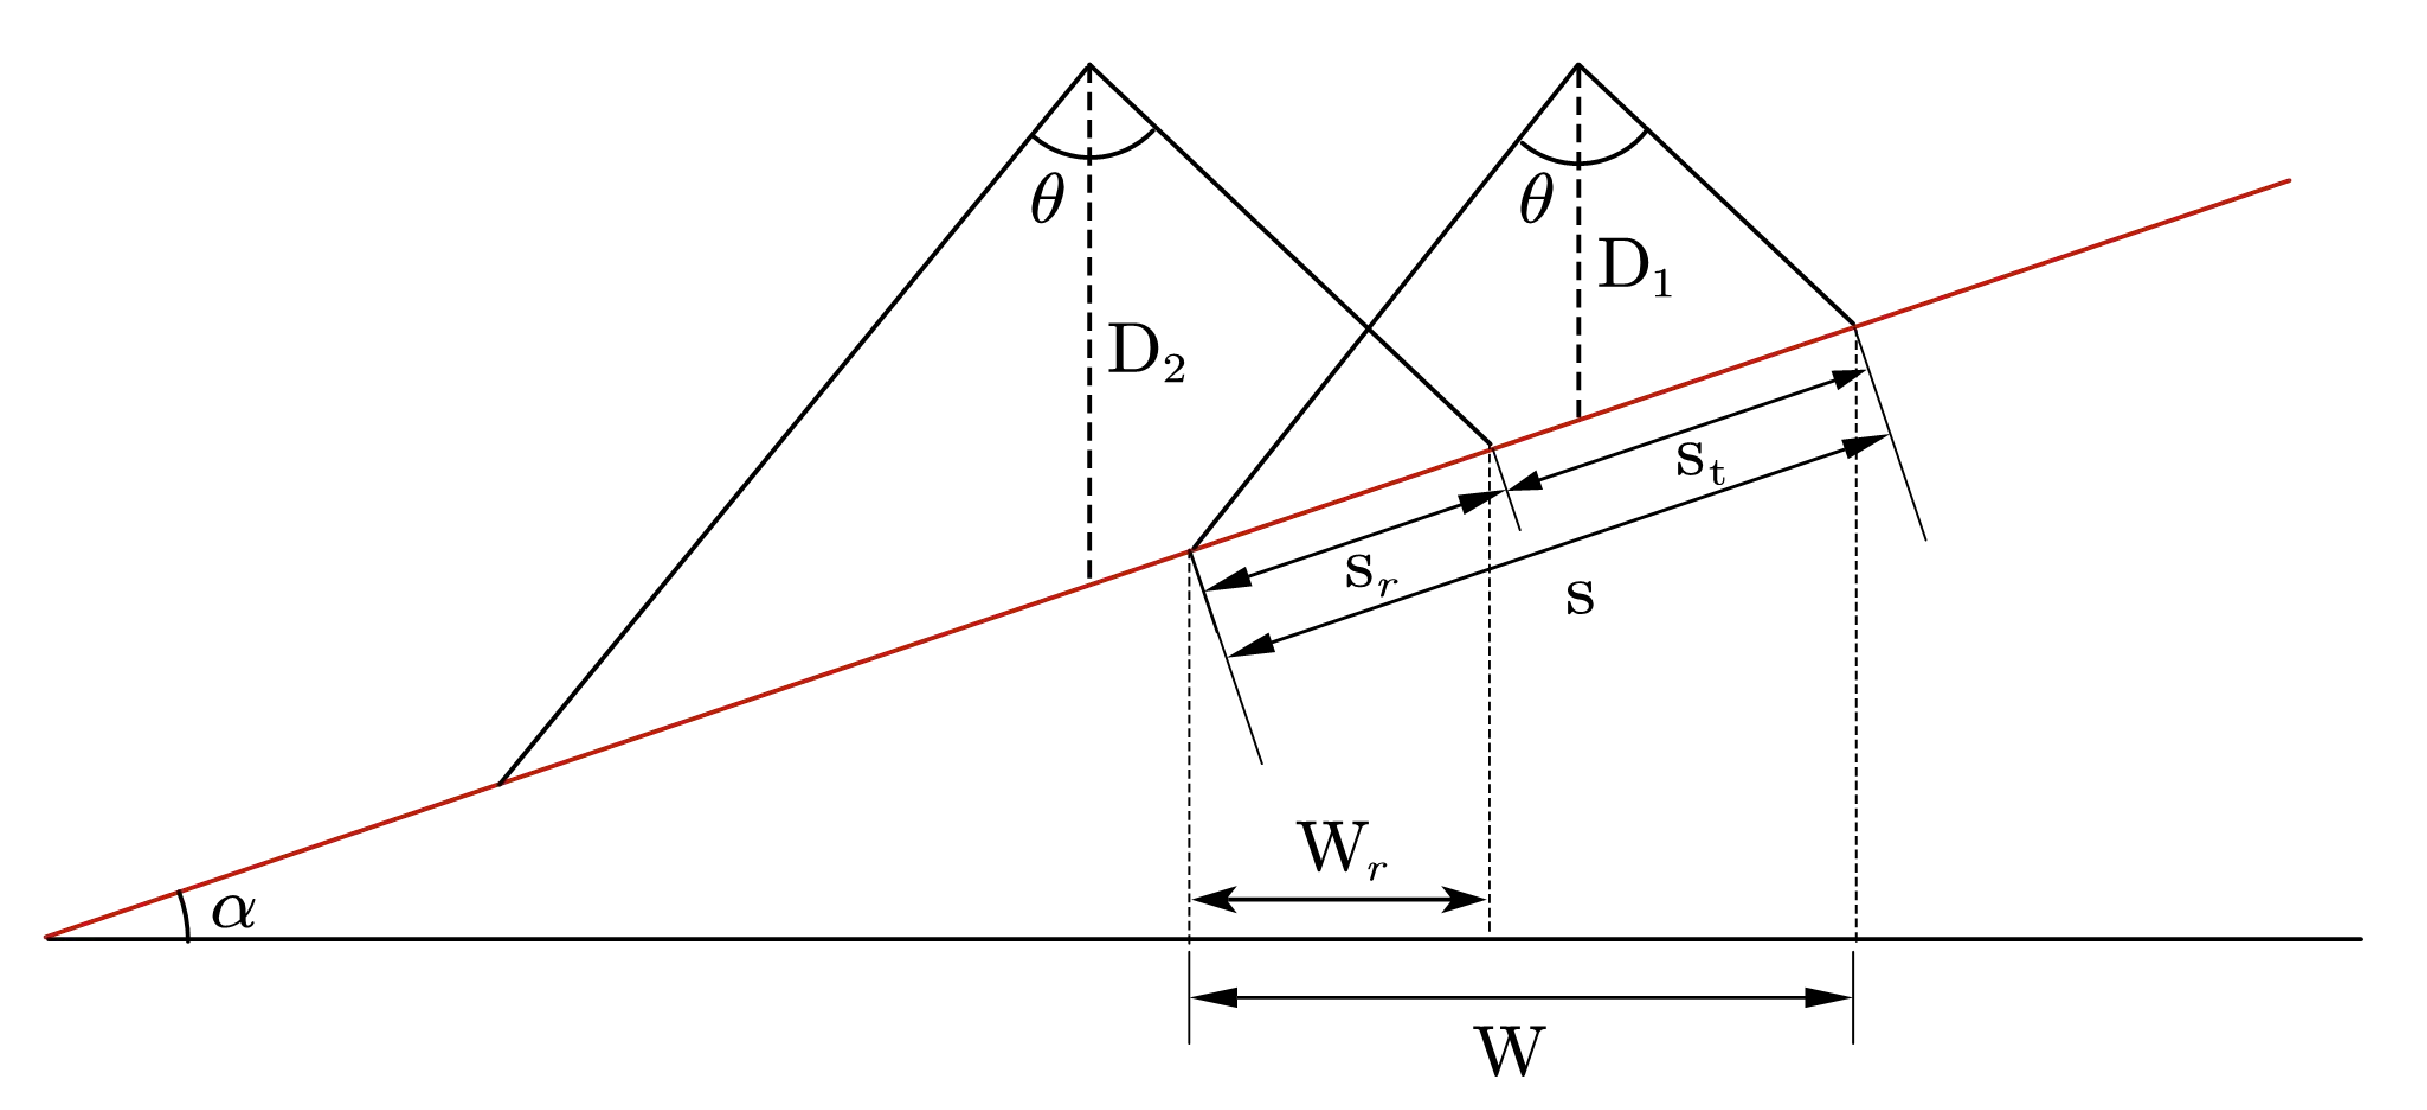
\includegraphics[width=.7\textwidth, height=14cm]{f2}
        \caption{算法流程图}
        \label{fig:algorithm}
    \end{figure}

    解得\textbf{问题一的部分答案}如下:

    \begin{figure}[H]
        \centering
        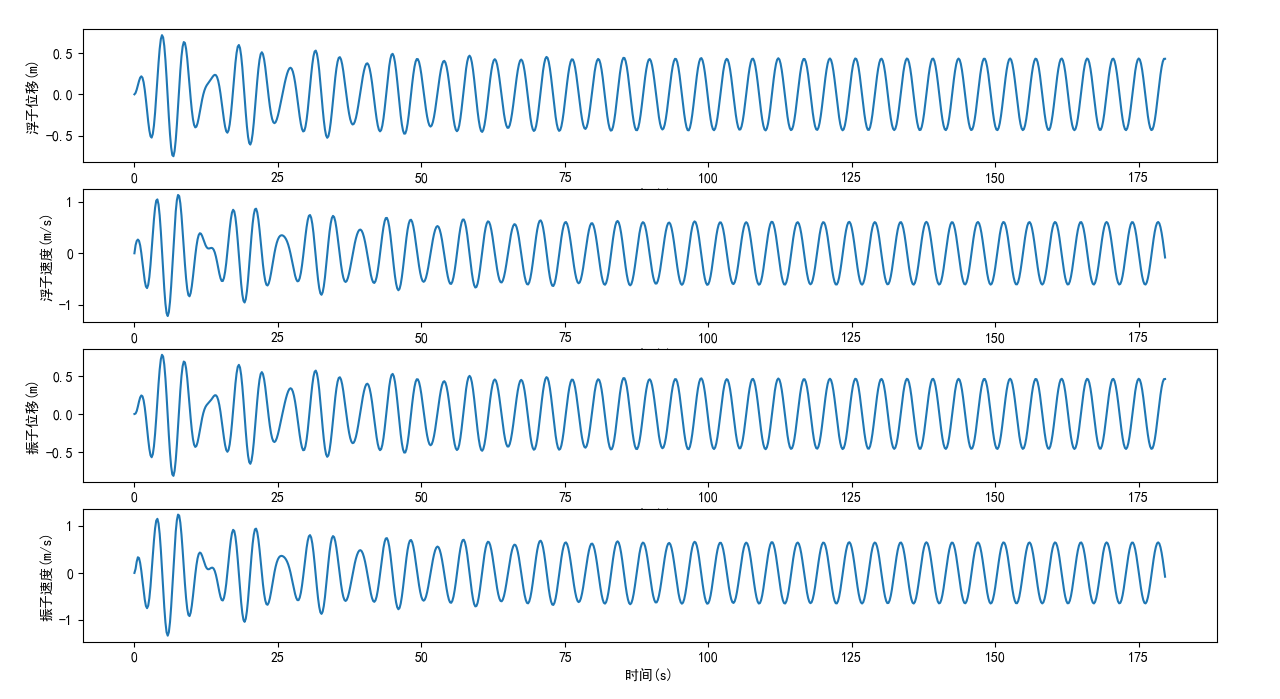
\includegraphics[width=.7\textwidth]{1_1}
        \caption{直线阻尼系数为常数时浮子与振子的垂荡位移和速度}
        \label{fig:1_1}
    \end{figure}

    \begin{figure}[H]
        \centering
        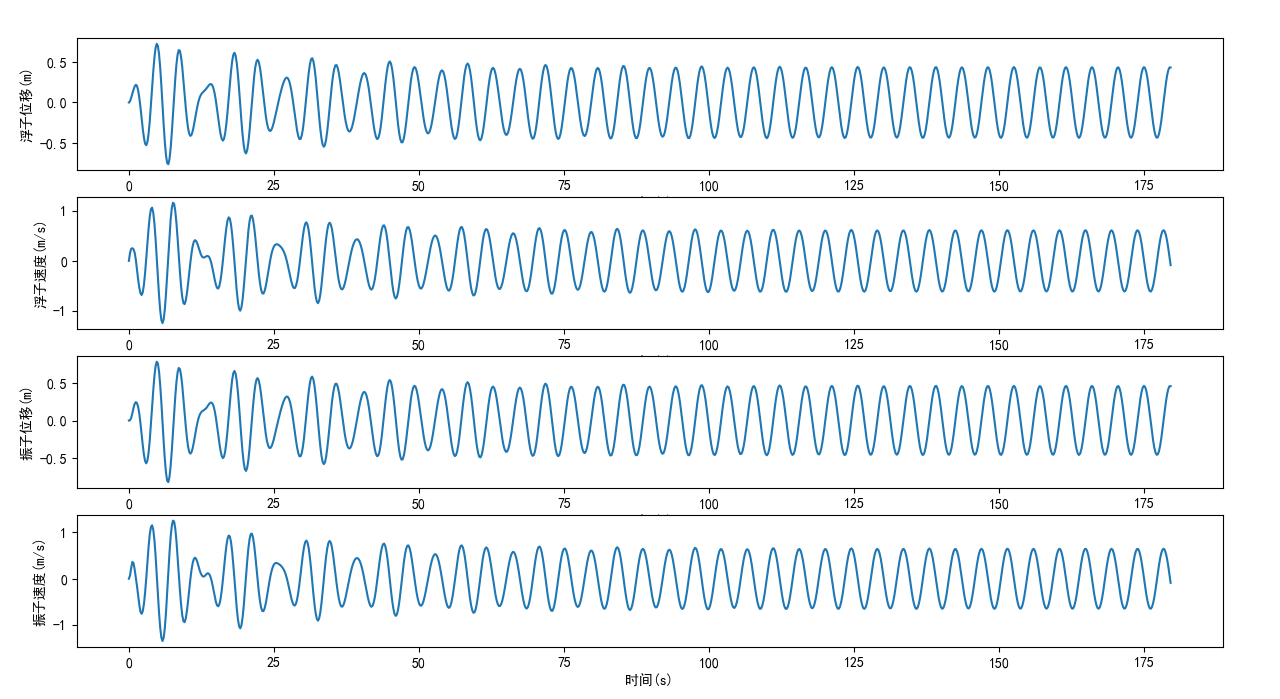
\includegraphics[width=.7\textwidth]{1_2}
        \caption{直线阻尼系数与相对速度成正比时浮子与振子的垂荡位移和速度}
        \label{fig:1_2}
    \end{figure}

    \begin{table}[H]
    \caption{题1.(1)部分结果展示}\label{tab:1.1} \centering
    \begin{tabular}{ccccc}
    \toprule[1.5pt]
    时间(s) & 浮子位移(m) & 浮子速度(m/s) & 振子位移(m) & 振子速度(m/s) \\
    \midrule[1pt]
    10 & -0.190917850969\ & -0.640171921322 & -0.209891792191 & -0.693490125224 \\
    20 &-0.590642700860 & -0.240396915234 & -0.632406132918 & -0.271166648214 \\
    40 &0.285335296034 & 0.313813255491 & 0.298469567943 & 0.333628990400 \\
    60 & -0.314438443527 & -0.478908125823 & -0.329510747194 & -0.515131086023 \\
    100 & -0.083615408956 & -0.603953625620 & -0.082100773522 & -0.642904159114 \\
    \bottomrule[1.5pt]
    \end{tabular}
    \end{table}

    \begin{table}[H]
        \caption{题1.(2)部分结果展示}\label{tab:1.2} \centering
        \begin{tabular}{ccccc}
        \toprule[1.5pt]
        时间(s) & 浮子位移(m) & 浮子速度(m/s) & 振子位移(m) & 振子速度(m/s) \\
        \midrule[1pt]
        10 & -0.203426228434 & -0.649403786522 & -0.227860620866 & -0.701458747351 \\
        20 & -0.607422582175 & -0.2509779588663 & -0.654201518714 & -0.279520027290 \\
        40 & 0.271699214007 & 0.297980728407 & 0.2854099275647 & 0.3156023096053 \\
        60 & -0.325034866537 & -0.4888934663089 & -0.344237375125 & -0.524781615969 \\
        100 & -0.087752670637 & -0.608840724257 & -0.0897244480920 & -0.648795785159 \\
        \bottomrule[1.5pt]
        \end{tabular}
        \end{table}

    \subsection{问题二模型的建立与求解}
    \subsubsection{模型的建立}
    先考虑常数阻尼系数的情况,沿用问题一中建立的模型,对任给的阻尼系数$ b $,可以得到新的参数设置下的$ z(t) $。
    仍令$ v = v_1 - v_2 $
    根据直线阻尼器的$ F-v $关系,可以得到直线阻尼器在$(t_0, t_0 + T)$内的平均功率表达式为
    \begin{equation}
        \overline{P} = \frac{1}{T}\int_{t_0}^{t_0 + T}bv(t)^2 dt
        \label{eq:ave_power_1}
    \end{equation}
    则由\cref{eq:wave}\cref{eq:G1}\cref{eq:G2}\cref{eq:d1}\cref{eq:d}\cref{eq:newton}\cref{eq:split_b}\cref{eq:split_e}\cref{eq:ave_power_1}可得到直线阻尼器阻尼系数的优化模型:

    \textbf{目标函数}:
    \begin{equation}
        arg \max_{b} \overline{P} = \frac{1}{T}\int_{t_0}^{t_0 + T}bv(t)^2 dt
        \label{eq:target_1}
    \end{equation}

    \textbf{约束条件}:
    \begin{equation}
        s.t.
        \begin{cases}
            v(t) = \dot{x1} - \dot{x2}\\
            G_1 + F_w + F_b + F_{d1} - F_e - F_d = (m_1 + m_3) \ddot{x_1}\\
            G_2 + F_e + F_d = m_2 \ddot{x_2}\\
            F_w = f \cos\omega t \\
            F_b = \rho g V_0 + \rho g \pi r_1^2 x_1\\
            G_1 = m_1 g\\
            G_2 = m_2 g\\
            F_{d1} = b_1\dot{x_1}\\
            F_e = k x_0 - k(x_2 - x_1)\\
            F_d = b(\dot{x_1} - \dot{x_2})\\
            0 \leq b \leq 100000 \\
        \end{cases}
        \label{eq:control_1}
    \end{equation}
    具体优化方法将在模型求解中讨论。

    接下来考虑直线阻尼器的阻尼系数与振子、浮子的相对速度的$p$次成正比的情况,$p \in[0, 1]$。
    仍使用问题二中的线性化方法,$ F_d = (1 + p) b_0 {\left| v_0 \right|}^p v - p b_0{\left| v_0 \right|}^ p v_0  $
    则$ A $和 $ u $更新为:
    $$
    A = \left [
        \begin{array}{cccc}
            0&1&0&0 \\
            \frac{-k -\rho g \pi r_1^2}{m_1 + m_3} & \frac{-b - b_1}{m_1 + m_3}
            & \frac{k}{m_1 + m_3} & \frac{b}{k1 + k3}\\
            0&0&0&1 \\
            \frac{k}{m_2}& \frac{b}{m_2} & \frac{-k}{m_2} & \frac{-b}{m_2}\\
        \end{array} \right ]
    $$其中,直线阻尼系数 $b = (1+p) b_0 |v|^p$。
    $$
    u = \left [
        \begin{array}{c}
            f\cos \omega t - m_1 g + \rho g V_0 - k x_0 - p b_0 |v_0|^{p}v_0\\
            -m_2 g + k x_0 + p b_0 |v_0|^{p}v_0 \\
        \end{array} \right ]
    $$
    仍沿用问题一中处理局部状态空间方程的迭代方法,则对任给的阻尼系数$ b_0 $ 与幂次$ p $可以解出$ z(t) $。

    此时,直线阻尼器在$(t_0, t_0 + T)$内的平均功率表达式为:
    \begin{equation}
        \overline{P} = \frac{1}{T}\int_{t_0}^{t_0 + T}bv(t)^{2+p} dt
        \label{eq:ave_power_2}
    \end{equation}
    由\cref{eq:wave}\cref{eq:G1}\cref{eq:G2}\cref{eq:d1}\cref{eq:d}\cref{eq:newton}\cref{eq:split_b}\cref{eq:split_e}\cref{eq:ave_power_2}可得到如下直线阻尼器阻尼系数的优化模型:

    \textbf{目标函数}:
    \begin{equation}
        arg \max_{b_0, p} \overline{P} = \frac{1}{T}\int_{t_0}^{t_0 + T}bv(t)^{2+p} dt
        \label{eq:target_2}
    \end{equation}

    \textbf{约束条件}:
    \begin{equation}
        s.t.
        \begin{cases}
            v = \dot{x1} - \dot{x2}\\
            G_1 + F_w + F_b + F_{d1} - F_e - F_d = (m_1 + m_3) \ddot{x_1}\\
            G_2 + F_e + F_d = m_2 \ddot{x_2}\\
            F_w = f \cos\omega t \\
            F_b = \rho g V_0 + \rho g \pi r_1^2 x_1\\
            G_1 = m_1 g\\
            G_2 = m_2 g\\
            F_{d1} = b_1\dot{x_1}\\
            F_e = k x_0 - k(x_2 - x_1)\\
            F_d = b(\dot{x_1} - \dot{x_2})\\
            b = b_0 v^p\\
            0 \leq b_0 \leq 100000 \\
            0 \leq p \leq 1\\
        \end{cases}
        \label{eq:control_2}
    \end{equation}
    具体优化方法将在模型求解中讨论。
    \subsubsection{模型的求解}
    由浮子、振子位移图像可知,前期位移不稳定,并且越往后位移稳定性越强,于是本文采用 $40$个周期内的后 $20s$ 来计算平均功率。 
    对于阻尼系数为常数的情况,由于该问题为单目标单变量优化问题,优先采用暴力搜索法求得最优阻尼系数。
    本文先采用增大步长的方式来得到粗略结果,令直线阻尼系数$b$步长为 $100$ 绘出平均功率 与 直线阻尼系数 $b$的图如\cref{fig:power_b}。
    \begin{figure}[!htbp]
        \centering
        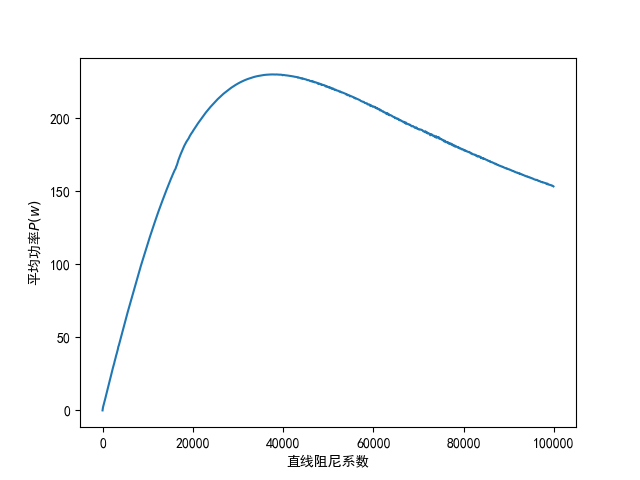
\includegraphics[width=.9\textwidth]{f3}
        \caption{平均功率与直线阻尼系数的关系}
        \label{fig:power_b}
    \end{figure}
    
    不难看出,平均功率与直线阻尼系数的函数大致上为凸函数,具有凸性,最优阻尼系数大致在 $30000 \sim 40000$ 之间,于是本题最终采用步长为 $1$ 的暴力搜索法来精确结果,求得\textbf{最大平均功率}为 $229.997w$,此时的\textbf{最优直线阻尼系数}为 $37993$。

    而对于直线阻尼器的阻尼系数与振子、浮子的相对速度的$p$次成正比的情况,由于该问题为单目标多变量优化问题,采用暴力搜索法时间较长,
    于是采用遗传算法来求解该问题。遗传算法是一种全局优化算法,能解决陷入局部最优解的死循环的问题,
    且搜索从群体出发,具有潜在的并行性,能快速找到答案。遗传算法的具体流程如\cref{fig:GA}。

    通过遗传算法,求得最大平均输出功率为$230.402w$,此时最优直线阻尼系数为$37779$,幂指数为 $0.0001$。

    \begin{figure}[H]
        \centering
        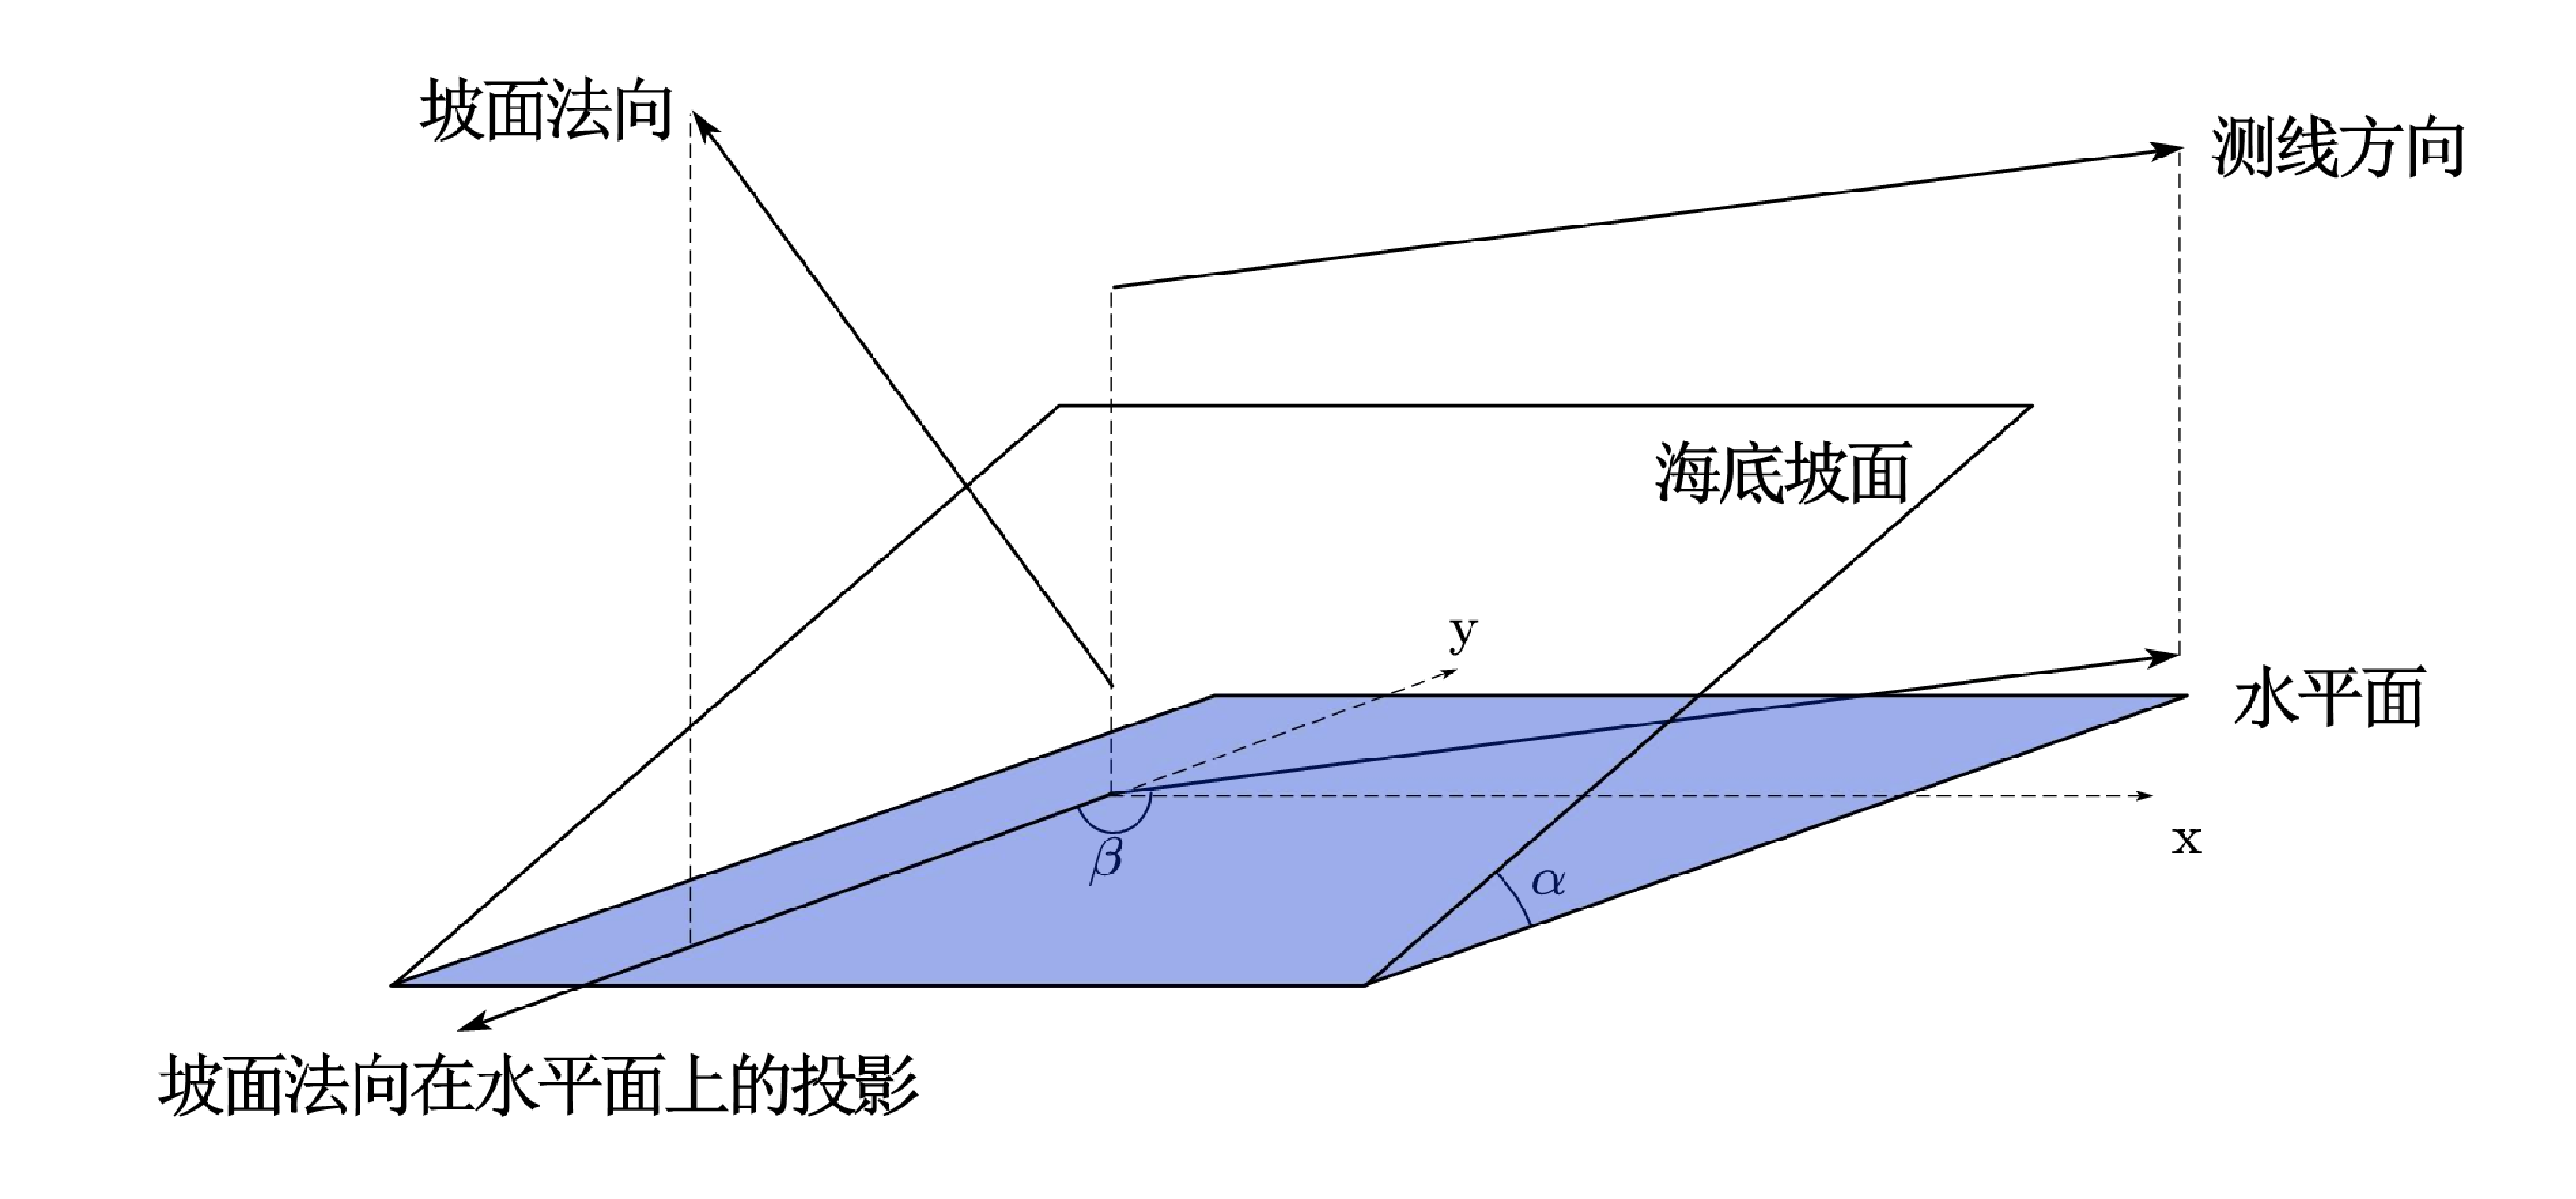
\includegraphics[width=.5\textwidth]{f4}
        \caption{遗传算法具体流程}
        \label{fig:GA}
    \end{figure}
    \subsection{问题三模型的建立与求解}
    \subsubsection{模型的建立}
    模型的建立
    \subsubsection{模型的求解}
    \begin{figure}[H]
        \centering
        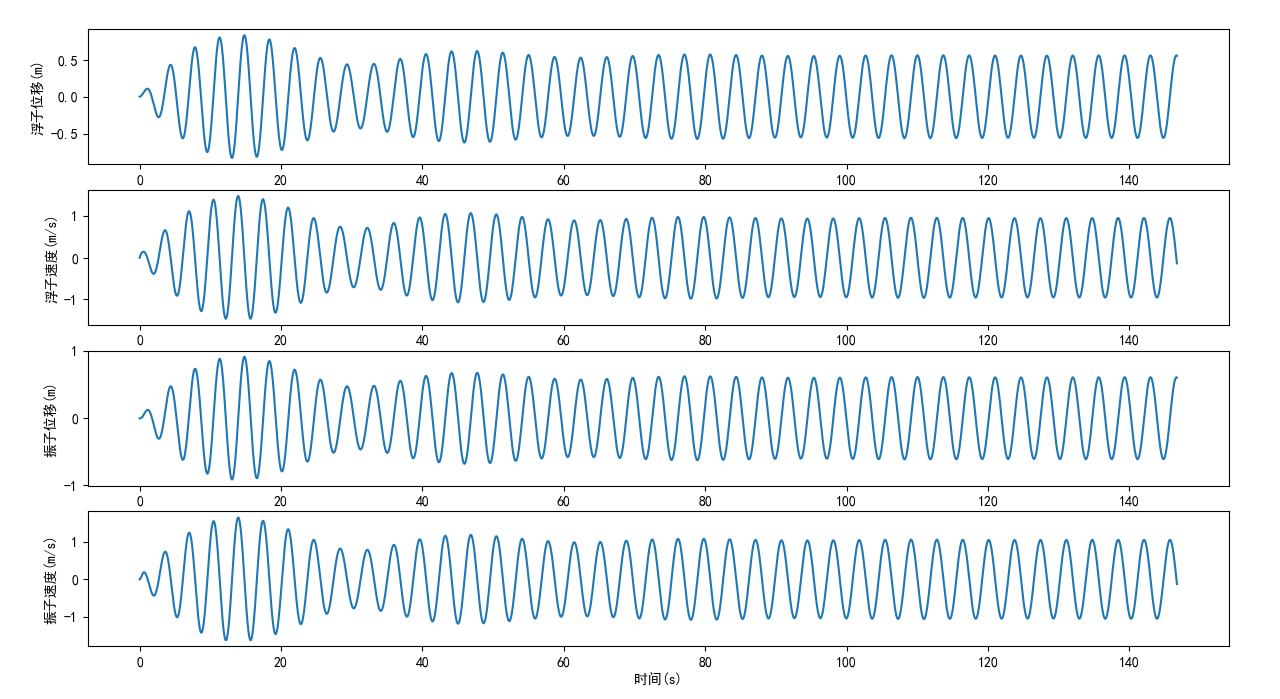
\includegraphics[width=.9\textwidth]{3_1}
        \caption{浮子与振子的垂荡位移和速度}
        \label{fig:3_1}
    \end{figure}

    \begin{figure}[H]
        \centering
        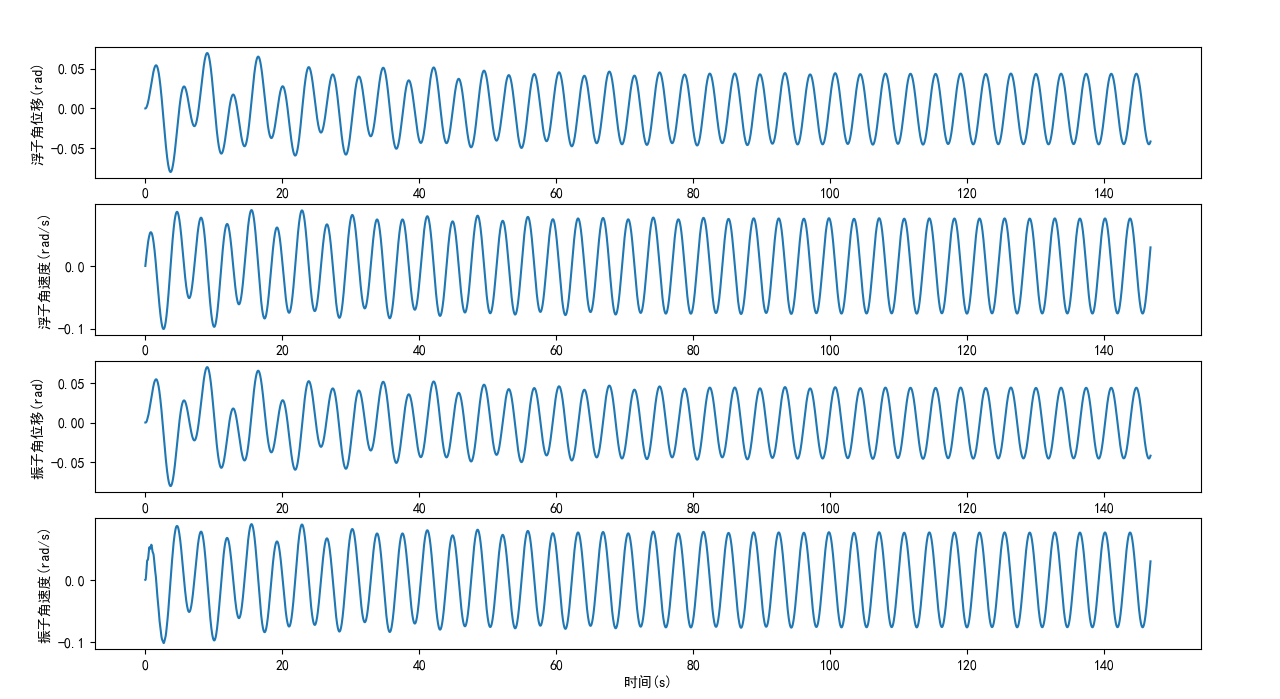
\includegraphics[width=.9\textwidth]{3_2}
        \caption{浮子与振子的垂荡角位移和角速度}
        \label{fig:3_2}
    \end{figure}

    \begin{table}[H]
        \caption{题3垂荡运动部分结果展示}\label{tab:3.1} \centering
        \begin{tabular}{ccccc}
        \toprule[1.5pt]
        时间(s) & 浮子位移(m) & 浮子速度(m/s) & 振子位移(m) & 振子速度(m/s) \\
        \midrule[1pt]
        10 & -0.528646475568 & 0.969906801905 & -0.597185543397 & 1.038245246333 \\
        20 & -0.705038971844 & -0.269153121495 & -0.770588011827 & -0.318865145333 \\
        40 & 0.369294946450 & 0.757715335051 & 0.3945357695949 & 0.845111641422 \\
        60 & -0.3206897596166 & -0.721694618283 & -0.339484605441 & -0.799246142172 \\
        100 & -0.0501596515299 & -0.946684151030 & -0.0406594668670 & -1.036519619445 \\
        \bottomrule[1.5pt]
        \end{tabular}
        \end{table}

    \begin{table}[H]
        \caption{题3纵摇运动部分结果展示}\label{tab:3.2} \centering
        \begin{tabular}{ccccc}
        \toprule[1.5pt]
        时间(s) & 浮子角位移(rad) & 浮子角速度(rad/s) & 振子角位移(rad) & 振子角速度(rad/s) \\
        \midrule[1pt]
        10 & 0.011811123210 & -0.096889918017 & 0.011840841660 & -0.097408836375 \\
        20 & 0.027660719280 & 0.005659312454 & 0.027930286000 & 0.005705657726 \\
        40 & -0.040421576717 & -0.026320884440 & -0.040773222383 & -0.026700178027 \\
        60 & 0.035729998823 & 0.047026278691 & 0.03599482267 & 0.047342729467 \\
        100 & 0.015334589710 & 0.071312953754 & 0.015465917718 & 0.071882896180 \\
        \bottomrule[1.5pt]
        \end{tabular}
        \end{table}
    \subsection{问题四模型的建立与求解}
    \subsubsection{模型的建立}
    问题四模型的建立
    \subsubsection{模型的求解}
    问题四模型的求解
    \newpage
    \section{模型的分析与检验}
    本文从以下三个方面对模型进行分析与检验:
    \subsection{参数灵敏度分析}
    本文建立的模型基于物理定律,(旋转/直线)阻尼系数、阻尼系数幂次等变量应认为是模型输入的一部分,
    兴波阻尼系数、附加质量等参数由题目给出,故暂时只对自行进行简化计算的浮子转动惯量进行灵敏度分析。
    本文给浮子转动惯量一个$ 1\% $的扰动,以平均输出功率作为输出反馈的度量。
    经计算,当给予浮子转动惯量一个 $+1\%$ 的扰动与一个 $-1\%$ 的扰动时,装置平均输出功率的变化值均为$0.0233w$,平均输出功率的相对误差 
    小于0.06 \%,变化不大,模型稳定性较强。
    
    \subsection{对初态扰动的稳定性分析}
    本文建立模型时,选取的状态量初值均为模型静态平衡时对应的值。
    而现实中的模型可能从任意状态开始运行,因此需要对模型对初态的稳定性进行检验。
    对初态的稳定性应有两种含义:
    1. 给模型的初始状态一个微小的扰动,模型输出的变化应当可控。
       以问题一、二中建立的模型为例,让模型的初值$ z_0 = [-2, 0, -1.8, 0] $ + 一个较小的正态噪声$\epsilon$,
       在该初值下求解模型,得到$ z_{\epsilon}(t) $与$ z(t) $应当较为相近。本文用
        $$
        \sqrt{\frac{1}{n}\sum\limits_{i=1}^n(\frac{z(i * \Delta t) - z_{\epsilon}(i * \Delta t)}{z(i * \Delta t)} )^2}
        $$
    来衡量$ z_{\epsilon}(t) $与$ z(t) $的在离散时间步上的平均相对误差
       作为相似性的度量。

       经检验,正态噪声均值为 $0$,方差为 $0.01$时, 在100次采样下$z$ 的平均相对误差为 $[0.007\%,0.48\%,0.014\%,2.5\%]$,可知平均相对误差在$3\%$范围内。

    2. 给模型的初始状态一个稍大的扰动,模型趋于稳定后平均输出功率的变化应当较不明显。
        
        以问题一、二中建立的模型为例,让模型的初值$ z_0 = [-2, 0, -1.8, 0] + $ 一个略大的正态噪声$\epsilon$,
        在该初值下求解模型,得到$ z_{\epsilon}(t) $。本文选取$ t \geq 20s $后$ z_{\epsilon}(t) $
        与$ z(t) $的 平均功率的差的绝对值与真实平均功率的比 $\frac{\Delta p}{p}$ 作为相似性的度量。

        经检验,正态噪声均值为 $0$,方差为 $1$时, 在100次采样 平均功率的平均相对误差为 $0.00016\%$,可知平均相对误差在$0.0002\%$范围内。

    综上,模型对初态扰动有较好的稳定性。
    \subsection{对部分原始假设的验证}
    对于假设6: 水面仅在浮子圆柱部分浮动,从而使浮力的变化可被浮子位置的变化线性表达。
    由 \cref{fig:1_1},\cref{fig:1_2},\cref{fig:3_1}可知,浮子垂荡位移小于 $1m$,该假设成立。

    对于假设7: 纵摇运动角度较小,对垂荡运动影响较小。
    由 \cref{fig:3_2} 可知,纵摇的角度小于 $0.1 rad$,可认为纵摇运动角度较小,该假设成立。
    \section{模型的评价、改进与推广}
    \subsection{模型的优点}
    \begin{enumerate}
        \item \textbf{机理支撑}:使用牛顿第二定律、刚体的定轴转动定律建立装置的垂荡和纵摇模型,和实际情形相近,有较为合理的描述了装置垂荡纵摇的运动情形。
        \item \textbf{模型简洁}:将多条力学方程转化为状态空间方程,简化了模型的求解,证明了解的存在性与唯一性,对部分问题给出了解析解,并基于解析解给出了精度可控的数值解。
        \item \textbf{灵活使用多种优化方法}:在优化变量数量较少时使用搜索方法,在优化变量数量较多时综合使用搜索法和遗传算法。
    \end{enumerate}
    \subsection{模型的缺点}
    \begin{enumerate}
        \item 以过于简单的方式处理了纵摇与垂荡之间的关系。在实际情况下纵摇和垂荡是相互影响的,但在本文建立的模型中只考虑了垂荡运动对纵摇运动的影响。
        \item 在建立装置纵摇运动模型时,忽略了振子重力矩的影响。
        \item 模型所需的假设较多:如纵摇的角度较小、外力矩参考轴过浮子质心等。
    \end{enumerate}
    \subsection{模型的改进}
    \begin{enumerate}
        \item 建立装置垂荡和纵摇的耦合运动模型,并在此基础上加以改进。
        \item 在纵摇运动模型上考虑更好的局部线性拟合方法。
    \end{enumerate}
    \subsection{模型的推广}
    本文基于二自由度弹簧阻尼模型的抽象建立了波浪能利用装置垂荡的运动模型,给出了一种有效的分析最优阻尼器参数的方法。
    因此,本文的工作可以被推广到其他含阻尼器模块的装置的分析,如电车中的含电磁阻尼器的电能回收装置等,用于优化装置中的阻尼器参数来达到预期效果。
    \newpage
    \begin{thebibliography}{9}%宽度9
        \bibitem[1]{Wave_energy_device_1}
        盛松伟,游亚戈,张亚群等.
        \newblock 一种点吸收式波浪能装置水动力学研究\allowbreak[J].
        \newblock 太阳能学报,2013,34(08):1443-1449.
        \bibitem[2]{Wave_energy_device_2}
        董晓晨,李德敏,史宏达.
        \newblock 同轴双浮体波能装置最优获能研究\allowbreak[J].
        \newblock 太阳能学报,2021,42(03):228-234.DOI:10.19912/j.0254-0096.tynxb.2021-0081.
        \bibitem[3]{Wave_energy_device_3}
        郑雄波,张亮,马勇.
        \newblock 双浮体波能装置的水动力计算与能量转换特性分析\allowbreak[J].
        \newblock 科技导报,2014,32(19):26-30.
    \end{thebibliography}

    \newpage
    \begin{appendices}
        \section{问题一}

        \begin{lstlisting}[language=python]
        # 第一小问

        import numpy as np
        from scipy.integrate import solve_ivp
        from numpy import fft
        import pylab as plt
        x0 = 0.5
        k = 80000
        m1 = 4866
        m2 = 2433
        b = 10000
        f = 6250
        omega = 1.4005
        g = 9.8
        pho = 1025
        r = 1
        V0 = 1/3 * np.pi * r * r * 0.8

        def buoyancy(h) -> float:
            '''根据浮子距离海平面位置, 返回相应浮力'''
            if h < 0:
                return 0
            elif h < 0.8:
                r =  h / 0.8
                V = 1/3 * np.pi * r * r * h
            elif 0.8 <= h < 3.8:
                r = 1
                V = V0 + np.pi * r * r * (h - 0.8)
            else:
                r = 1
                V = V0 + np.pi * r * r * 3
            return pho * g * V

        def pd_toexcel(data,filename): # pandas库储存数据到excel
            dfData = { # 用字典设置DataFrame所需数据
            '时间':data[0],
            '浮子位移':data[1],
            '浮子速度':data[2],
            '振子位移':data[3],
            '振子速度':data[4],
            }
            df = pd.DataFrame(dfData) # 创建DataFrame
            #用openpyxl打开excel
            wb=openpyxl.load_workbook(filename)
            #打开指定的Sheet
            ws = wb['Sheet1']
            
            startCol = 1
            startRow = 3
            
            #下面两行的意思是,将df1的每一行转成列表
            for i in range(0, df.shape[0]):
                eachRowList = df.iloc[i,:].tolist()
                #取每个列表里面的值
                for j in range(0,len(eachRowList)):
                    #row 代表从几行开始, columns 代表从第几列开始
                    ws.cell(row = startRow+i, column = startCol+j).value =eachRowList[j]
            
            #保存为新的表格
            wb.save(filename)

        def solve(b, m3, f, omega, b1):
            A = np.array([[0, 1, 0, 0], 
                        [-(k+pho * g * np.pi)/(m1+m3), -(b + b1)/(m1+m3), k/(m1+m3), b/(m1+m3)], 
                        [0, 0, 0, 1], 
                        [k/m2, b/m2, -k/m2, -b/m2]])
            B = np.array([[0, 0], 
                        [1/(m1+m3), 0], 
                        [0, 0],
                        [0, 1/m2]])

            def func(t, x):
                u = np.array([f*np.cos(omega*t) - m1 * g + pho * g * V0 - k * x0, - m2 * g + k * x0])
                return [np.dot(A[i, :], x) + np.dot(B[i, :], u) for i in range(4)]

            N = (2 * np.pi / omega) * 40 + 0.2
            t_span = (0, N)
            t_eval = np.arange(0, N, 0.01)
            y0 = [-2.0, 0, -1.8, 0]

            sol = solve_ivp(func, t_span, y0, t_eval=t_eval)
            return sol
            
        if __name__ == '__main__':
            sol = solve(b=10000, m3=1335.535, f=6250, omega=1.4005, b1=656.3616)
            data = np.zeros([5,len(sol.t.T)])
            data[0] = sol.t.T
            for i in range(0,4):
                if i == 0:
                    data[i+1] = sol.y[i,:] + 2 
                elif i == 2:
                    data[i+1] = sol.y[i,:] + 1.8 
                else:
                    data[i+1] = sol.y[i,:]
            # print(data)
            # pd_toexcel(data, 'result1-1.xlsx')
            # sol = solve(m3=1028.876, f=3640, omega=1.7152, b=10000, b1=683.4558)
            plt.rc('font',family='SimHei')
            plt.rc('axes', unicode_minus=False)
            plt.subplot(411)
            plt.plot(sol.t, sol.y.T[:, 0]+2)
            plt.xlabel('时间(s)')
            plt.ylabel('浮子位移(m)')
            plt.subplot(412)
            plt.plot(sol.t, sol.y.T[:, 1])
            plt.xlabel('时间(s)')
            plt.ylabel('浮子速度(m/s)')
            plt.subplot(413)
            plt.plot(sol.t, sol.y.T[:, 2]+1.8)
            plt.xlabel('时间(s)')
            plt.ylabel('振子位移(m)')
            plt.subplot(414)
            plt.plot(sol.t, sol.y.T[:, 3])
            plt.xlabel('时间(s)')
            plt.ylabel('振子速度(m/s)')
            print(sol.y.T[1000, 0] + 2, sol.y.T[1000, 1], sol.y.T[1000, 2] + 1.8, sol.y.T[1000, 3])
            print(sol.y.T[2000, 0] + 2, sol.y.T[2000, 1], sol.y.T[2000, 2] + 1.8, sol.y.T[2000, 3])
            print(sol.y.T[4000, 0] + 2, sol.y.T[4000, 1], sol.y.T[4000, 2] + 1.8, sol.y.T[4000, 3])
            print(sol.y.T[6000, 0] + 2, sol.y.T[6000, 1], sol.y.T[6000, 2] + 1.8, sol.y.T[6000, 3])
            print(sol.y.T[10000, 0] + 2, sol.y.T[10000, 1], sol.y.T[10000, 2] + 1.8, sol.y.T[10000, 3])
            plt.show()

        # 第二小问

        import numpy as np
        from scipy.integrate import solve_ivp
        import pylab as plt
        from question1_1 import pd_toexcel
        
        x0 = 0.5
        k = 80000
        m1 = 4866
        m2 = 2433
        g = 9.8
        rho = 1025
        r = 1
        V0 = 1/3 * np.pi * r * r * 0.8 
        
        def solve_step(z:list, t_start, m3, omega, f, b0:float, p:float, b1:float)->list:
            dv = z[1] - z[3]
            b = (p+1) * b0 * abs(dv) ** p
        
            A = np.array([[0, 1, 0, 0], 
                            [-(k+rho * g * np.pi)/(m1+m3), -(b + b1)/(m1+m3), k/(m1+m3), b/(m1+m3)], 
                            [0, 0, 0, 1], 
                            [k/m2, b/m2, -k/m2, -b/m2]])
            B = np.array([[0, 0], 
                            [1/(m1+m3), 0], 
                            [0, 0], 
                            [0, 1/m2]])
        
            def func(t, x):
                u = np.array([f*np.cos(omega*t) - m1 * g + rho * g * V0 - (p * b0 * abs(dv) ** (p+1)) - k * x0, - m2 * g + (p * b0 * abs(dv) ** (p+1)) + k * x0])
                return [np.dot(A[i, :], x) + np.dot(B[i, :], u) for i in range(4)]
        
            dt = 0.01
            t_span = (t_start, t_start + 2 * dt)
            t_eval = np.arange(t_start, t_start + 2 * dt, 0.01)
        
            sol = solve_ivp(func, t_span, z, t_eval=t_eval)
            return sol.y.T[1]
        
        def solve_all(x1, v1, x2, v2, m3, omega, f, b0:float, p:float, b1:float):
            t = 0
            while t < (2 * np.pi / omega * 40 + 0.2):
                z = [x1[-1], v1[-1], x2[-1], v2[-1]]
                z = solve_step(z, t, m3, omega, f, b0, p, b1)
                t += 0.01
                x1 = np.append(x1,z[0])
                v1 = np.append(v1,z[1])
                x2 = np.append(x2,z[2])
                v2 = np.append(v2,z[3])
            return x1,v1,x2,v2
        

        if __name__ == '__main__':
            omega = 1.4005
            z0 = [-2, 0, -1.8, 0]
            x1 = np.array([-2])
            v1 = np.array([0])
            x2 = np.array([-1.8])
            v2 = np.array([0])
            x1, v1, x2, v2 = solve_all(x1, v1, x2, v2, m3=1335.535, f=6250, omega=1.4005, b0=10000, p=0.5, b1=656.3616)
            t = np.arange(0, (2 * np.pi / omega) * 40 + 0.2+0.01, 0.01)
            t1 = [t[i] for i in range(0, len(t), 20)]
            x1_1 = [x1[i] + 2 for i in range(0, len(t), 20)]
            v1_1 = [v1[i] for i in range(0, len(t), 20)]
            x2_1 = [x2[i] + 1.8 for i in range(0, len(t), 20)]
            v2_1 = [v2[i] for i in range(0, len(t), 20)]
            data = np.zeros([5,len(t1)])
            data[0] = t1
            data[1] = x1_1
            data[2] = v1_1
            data[3] = x2_1
            data[4] = v2_1
            # print(data)
            # pd_toexcel(data, 'result1-2.xlsx')
            plt.rc('font',family='SimHei')
            plt.rc('axes', unicode_minus=False)
            plt.subplot(411)
            plt.plot(data[0], data[1])
            plt.xlabel('时间(s)')
            plt.ylabel('浮子位移(m)')
            plt.subplot(412)
            plt.plot(data[0], data[2])
            plt.xlabel('时间(s)')
            plt.ylabel('浮子速度(m/s)')
            plt.subplot(413)
            plt.plot(data[0], data[3])
            plt.xlabel('时间(s)')
            plt.ylabel('振子位移(m)')
            plt.subplot(414)
            plt.plot(data[0], data[4])
            plt.xlabel('时间(s)')
            plt.ylabel('振子速度(m/s)')
            print(x1[1000] + 2, v1[1000], x2[1000] + 1.8, v2[1000])
            print(x1[2000] + 2, v1[2000], x2[2000] + 1.8, v2[2000])
            print(x1[4000] + 2, v1[4000], x2[4000] + 1.8, v2[4000])
            print(x1[6000] + 2, v1[6000], x2[6000] + 1.8, v2[6000])
            print(x1[10000] + 2, v1[10000], x2[10000] + 1.8, v2[10000])
            plt.show()
                     
        \end{lstlisting}

        \section{问题二}

        \begin{lstlisting}[language=python]
        # 第一小问
        
        from question1_1 import solve
        from scipy.integrate import solve_ivp
        import numpy as np
        import pylab as plt

        x0 = 0.5
        k = 80000
        m1 = 4866
        m2 = 2433
        m3 = 1165.992
        f = 4890
        omega = 2.2143
        g = 9.8
        pho = 1025
        r = 1
        V0 = 1/3 * np.pi * r * r * 0.8

        def ave_power(b):
            sol = solve(b, m3=1165.992, f=4890, omega=2.2143, b1=167.8395)
            y = b * (sol.y.T[:, 1] - sol.y.T[:, 3]) ** 2
            all_power = 0
            for i in range(len(y) - 2001, len(y) - 1):
                all_power += (y[i] + y[i+1]) * 0.01 / 2
            ave_power = all_power / (2000 * 0.01)
            return ave_power

        if __name__ == '__main__':
            print(ave_power(37993))
            all_b = np.arange(0, 100000, 100)
            max = 0
            max_b = 0
            ave_power_list = []
            for b in all_b:
                ave_power_list.append(ave_power(b))
                print(b, ave_power(b))
                if(ave_power(b) > max):
                    max = ave_power(b)
                    max_b = b
            print('max:', max) # 229.99660485887816
            print("max_b", max_b) # 37993
            plt.rc('font', family='SimHei') # 用于正常显示中文标签 
            plt.plot(all_b, ave_power_list)
            plt.xlabel('直线阻尼系数')
            plt.ylabel('平均功率$P(w)$')
            plt.show()
        
        # 第二小问
        from question1_2 import solve_all
        import numpy as np
        from sko.GA import GA
        import matplotlib.pyplot as plt
        import pandas as pd

        def ave_power(x):
            """定义目标函数"""
            b, p = x
            x1 = np.array([-2])
            v1 = np.array([0])
            x2 = np.array([-1.8])
            v2 = np.array([0])
            x1, v1, x2, v2 = solve_all(x1, v1, x2, v2, m3=1165.992, omega=2.2143, f=4890, b0=b * 1e5, p=p, b1=167.8395)
            y = b * 1e5 * np.abs(v1 - v2) ** (2 + p)
            all_power = 0
            for i in range(len(y) - 2001, len(y) - 1):
                all_power += (y[i] + y[i+1]) * 0.01 / 2
            ave_power = all_power / (2000 * 0.01)
            return -ave_power # GA默认求最小值,加负号

        ga = GA(func=ave_power, n_dim=2, size_pop=200, max_iter=20, prob_mut=0.001, lb=[0.35, 0], ub=[0.45, 0.05], precision=1e-7)
        best_x, best_y = ga.run()
        print('best_x:', best_x, '\n', 'best_y:', best_y)

        Y_history = pd.DataFrame(ga.all_history_Y)
        fig, ax = plt.subplots(2, 1)
        ax[0].plot(Y_history.index, Y_history.values, '.', color='red')
        Y_history.min(axis=1).cummin().plot(kind='line')
        plt.show()
        \end{lstlisting}   

        \section{问题三}
        \begin{lstlisting}[language=python]
        import numpy as np
        from scipy.integrate import solve_ivp
        import pylab as plt
        
        x0 = 0.5 # 弹簧原长
        k = 80000 # 直线弹簧刚度
        m1 = 4866 # 浮子质量
        m2 = 2433 # 振子质量
        g = 9.8 # 重力加速度
        rho = 1025 # 密度
        r = 1 # 底面表面积
        h = 0.5 # 振子高度
        r1 = 0.5 # 振子半径
        V0 = 1/3 * np.pi * r * r * 0.8 # 圆锥体积
        L0 = 1.4 # 浮子质心到地面的距离
        K1 = 250000 # 扭转弹簧刚度
        K2 = 8890.7 # 静水力矩恢复系数
        J1 = 8289.43

        def pd_toexcel(data,filename): # pandas库储存数据到excel
            dfData = { # 用字典设置DataFrame所需数据
            '时间':data[0],
            '浮子位移':data[1],
            '浮子速度':data[2],
            '浮子角位移':data[3],
            '浮子角速度':data[4],
            '振子位移':data[5],
            '振子速度':data[6],
            '振子角位移':data[7],
            '振子角速度':data[8],
            }
            df = pd.DataFrame(dfData) # 创建DataFrame
            #用openpyxl打开excel
            wb=openpyxl.load_workbook(filename)
            #打开指定的Sheet
            ws = wb['Sheet1']
            
            startCol = 1
            startRow = 3
            
            #下面两行的意思是,将df1的每一行转成列表
            for i in range(0, df.shape[0]):
                eachRowList = df.iloc[i,:].tolist()
                #取每个列表里面的值
                for j in range(0,len(eachRowList)):
                    #row 代表从几行开始, columns 代表从第几列开始
                    ws.cell(row = startRow+i, column = startCol+j).value =eachRowList[j]
            
            #保存为新的表格
            wb.save(filename)
        
        def solve_step(z1:list, z2:list, t_start, m3, J3, omega, f, L, b1:float, B1:float, b0:float, B0:float)->list:
            b = b0
            L1 = z1[2] - z1[0] + h / 2 # 振子质心到转轴距离
            J2 = m2 * (L1 ** 2) + m2 * (h ** 2 / 12 + r1 ** 2 / 4) # 振子的转动惯量
        
            A = np.array([[0, 1, 0, 0], 
                            [-(k+rho * g * np.pi)/(m1+m3), -(b + b1)/(m1+m3), k/(m1+m3), b/(m1+m3)], 
                            [0, 0, 0, 1], 
                            [k/m2, b/m2, -k/m2, -b/m2]])
            B = np.array([[0, 0], 
                            [1/(m1+m3), 0], 
                            [0, 0], 
                            [0, 1/m2]])
            
            C = np.array([[0, 1, 0, 0],
                        [-(K1 + K2)/ (J1 + J3), -(B0 + B1) / (J1 + J3), K1 / (J1 + J3), B0 /(J1 + J3)],
                        [0, 0, 0, 1],
                        [K1 / J2, B0 / J2, (-K1)/ J2, -B0 / J2]])
            
            D = np.array([[0, 0], 
                        [1/(J1+J3), 0], 
                        [0, 0], 
                        [0, 1/J2]])
        
            def func1(t, x):
                u1 = np.array([f*np.cos(omega*t) - m1 * g + rho * g * V0 - k * x0, - m2 * g + k * x0])
                return [np.dot(A[i, :], x) + np.dot(B[i, :], u1) for i in range(4)]
            
            def func2(t, x):
                u2 = np.array([L * np.cos(omega * t), 0])
                return [np.dot(C[i, :], x) + np.dot(D[i, :], u2) for i in range(4)]
        
            dt = 0.01
            t_span = (t_start, t_start + 2 * dt)
            t_eval = np.arange(t_start, t_start + 2 * dt, 0.01)
        
            sol1 = solve_ivp(func1, t_span, z1, t_eval=t_eval)
            sol2 = solve_ivp(func2, t_span, z2, t_eval=t_eval)
            return sol1.y.T[1], sol2.y.T[1]
        
        def solve_all(x1, v1, x2, v2, theta1, omega1, theta2, omega2, m3, J3, omega, f, L, b1:float, B1:float, b0:float, B0:float):
            t = 0
            while t < (2 * np.pi / omega * 40 + 0.2):
                z1 = [x1[-1], v1[-1], x2[-1], v2[-1]]
                z2 = [theta1[-1], omega1[-1], theta2[-1], omega2[-1]]
                z1, z2 = solve_step(z1, z2, t, m3, J3, omega, f, L, b1, B1, b0, B0)
                t += 0.01
                x1 = np.append(x1,z1[0])
                v1 = np.append(v1,z1[1])
                x2 = np.append(x2,z1[2])
                v2 = np.append(v2,z1[3])
                theta1 = np.append(theta1, z2[0])
                omega1 = np.append(omega1, z2[1])
                theta2 = np.append(theta2, z2[2])
                omega2 = np.append(omega2, z2[3])
            return x1,v1,x2,v2,theta1, omega1, theta2, omega2
        
        if __name__ == '__main__':
            omega = 1.7152
            x1 = np.array([-2])
            v1 = np.array([0])
            x2 = np.array([-1.8])
            v2 = np.array([0])
            theta1 = np.array([0])
            omega1 = np.array([0])
            theta2 = np.array([0])
            omega2 = np.array([0])
            x1, v1, x2, v2, theta1, omega1, theta2, omega2 = solve_all(x1, v1, x2, v2, theta1, omega1, theta2, omega2, m3=1028.876, J3=7001.914, omega=1.7152, f=3640, L=1690, b1=683.4558, B1=654.3383 * 2, b0=10000, B0=1000)
            t = np.arange(0, (2 * np.pi / omega) * 40 + 0.2 + 0.01, 0.01)
            print(x1[1000]+2, v1[1000], x2[1000]+1.8, v2[1000])
            print(x1[2000]+2, v1[2000], x2[2000]+1.8, v2[2000])
            print(x1[4000]+2, v1[4000], x2[4000]+1.8, v2[4000])
            print(x1[6000]+2, v1[6000], x2[6000]+1.8, v2[6000])
            print(x1[10000]+2, v1[10000], x2[10000]+1.8, v2[10000])
            print(theta1[1000], omega1[1000], theta2[1000], omega2[1000])
            print(theta1[2000], omega1[2000], theta2[2000], omega2[2000])
            print(theta1[4000], omega1[4000], theta2[4000], omega2[4000])
            print(theta1[6000], omega1[6000], theta2[6000], omega2[6000])
            print(theta1[10000], omega1[10000], theta2[10000], omega2[10000])
            plt.rc('font',family='SimHei')
            plt.rc('axes', unicode_minus=False)
            plt.figure()
            plt.subplot(411)
            plt.plot(t, x1+2)
            plt.xlabel('时间(s)')
            plt.ylabel('浮子位移(m)')
            plt.subplot(412)
            plt.plot(t, v1)
            plt.xlabel('时间(s)')
            plt.ylabel('浮子速度(m/s)')
            plt.subplot(413)
            plt.plot(t, x2+1.8)
            plt.xlabel('时间(s)')
            plt.ylabel('振子位移(m)')
            plt.subplot(414)
            plt.plot(t, v2)
            plt.xlabel('时间(s)')
            plt.ylabel('振子速度(m/s)')
            plt.figure()
            plt.subplot(411)
            plt.plot(t, theta1)
            plt.xlabel('时间(s)')
            plt.ylabel('浮子角位移(rad)')
            plt.subplot(412)
            plt.plot(t, omega1)
            plt.xlabel('时间(s)')
            plt.ylabel('浮子角速度(rad/s)')
            plt.subplot(413)
            plt.plot(t, theta2)
            plt.xlabel('时间(s)')
            plt.ylabel('振子角位移(rad)')
            plt.subplot(414)
            plt.plot(t, omega2)
            plt.xlabel('时间(s)')
            plt.ylabel('振子角速度(rad/s)')
            plt.show()
        \end{lstlisting}

        \section{问题四}
        \begin{lstlisting}[language=python]
        import numpy as np
        from question3 import solve_all
        from sko.GA import GA
        import matplotlib.pyplot as plt
        import pandas as pd
        from sko.tools import set_run_mode

        def ave_power(x):
            """定义目标函数"""
            b0, B0 = x
            x1 = np.array([-2])
            v1 = np.array([0])
            x2 = np.array([-1.8])
            v2 = np.array([0])
            theta1 = np.array([0])
            omega1 = np.array([0])
            theta2= np.array([0])
            omega2 = np.array([0])
            x1, v1, x2, v2, theta1, omega1, theta2, omega2 = solve_all(x1, v1, x2, v2, theta1, omega1, theta2, omega2, m3=1091.099, J3=7142.493, omega=1.9806, f=1760, L=2140, b1=528.5018, B1=1655.909, b0=b0, B0=B0)
            y1 = b0 * np.abs(v1 - v2) ** 2
            y2 = B0 * np.abs(omega1 - omega2) ** 2
            all_power = 0
            for i in range(len(y1) - 2001, len(y1) - 1):
                all_power += (y1[i] + y1[i+1]) * 0.01 / 2 + (y2[i] + y2[i+1]) * 0.01 / 2
            ave_power = all_power / (2000 * 0.01)
            return -ave_power # GA默认求最小值,加负号

        set_run_mode(ave_power, 'parallel')
        ga = GA(func=ave_power, n_dim=2, size_pop=200, max_iter=20, prob_mut=0.001, lb=[55000, 0], ub=[65000, 100000], precision=1e-7)
        best_x, best_y = ga.run()
        print('best_x:', best_x, '\n', 'best_y:', best_y)

        Y_history = pd.DataFrame(ga.all_history_Y)
        fig, ax = plt.subplots(2, 1)
        ax[0].plot(Y_history.index, Y_history.values, '.', color='red')
        Y_history.min(axis=1).cummin().plot(kind='line')
        plt.show()

        \end{lstlisting}

        \section{参数灵敏度分析}
        \begin{lstlisting}[language=python]
        import numpy as np
        from scipy.integrate import solve_ivp
        import pandas as pd
        import openpyxl

        x0 = 0.5 # 弹簧原长
        k = 80000 # 直线弹簧刚度
        m1 = 4866 # 浮子质量
        m2 = 2433 # 振子质量
        g = 9.8 # 重力加速度
        rho = 1025 # 密度
        r = 1 # 底面表面积
        h = 0.5 # 振子高度
        r1 = 0.5 # 振子半径
        V0 = 1/3 * np.pi * r * r * 0.8 # 圆锥体积
        L0 = 1.4 # 浮子质心到地面的距离
        K1 = 250000 # 扭转弹簧刚度
        K2 = 8890.7 # 静水力矩恢复系数
        J1 = 8289.43

        def pd_toexcel(data,filename): # pandas库储存数据到excel
            dfData = { # 用字典设置DataFrame所需数据
            '时间':data[0],
            '浮子位移':data[1],
            '浮子速度':data[2],
            '浮子角位移':data[3],
            '浮子角速度':data[4],
            '振子位移':data[5],
            '振子速度':data[6],
            '振子角位移':data[7],
            '振子角速度':data[8],
            }
            df = pd.DataFrame(dfData) # 创建DataFrame
            #用openpyxl打开excel
            wb=openpyxl.load_workbook(filename)
            #打开指定的Sheet
            ws = wb['Sheet1']
            
            startCol = 1
            startRow = 3
            
            #下面两行的意思是,将df1的每一行转成列表
            for i in range(0, df.shape[0]):
                eachRowList = df.iloc[i,:].tolist()
                #取每个列表里面的值
                for j in range(0,len(eachRowList)):
                    #row 代表从几行开始, columns 代表从第几列开始
                    ws.cell(row = startRow+i, column = startCol+j).value =eachRowList[j]
            
            #保存为新的表格
            wb.save(filename)

        def solve_step(z1:list, z2:list, t_start, m3, J3, omega, f, L, b1:float, B1:float, b0:float, B0:float)->list:
            b = b0
            L1 = z1[2] - z1[0] + h / 2 # 振子质心到转轴距离
            J2 = m2 * (L1 ** 2) + m2 * (h ** 2 / 12 + r1 ** 2 / 4) # 振子的转动惯量

            A = np.array([[0, 1, 0, 0], 
                        [-(k+rho * g * np.pi)/(m1+m3), -(b + b1)/(m1+m3), k/(m1+m3), b/(m1+m3)], 
                        [0, 0, 0, 1], 
                        [k/m2, b/m2, -k/m2, -b/m2]])
            B = np.array([[0, 0], 
                        [1/(m1+m3), 0], 
                        [0, 0], 
                        [0, 1/m2]])
            
            C = np.array([[0, 1, 0, 0],
                    [-(K1 + K2)/ (J1 + J3), -(B0 + B1) / (J1 + J3), K1 / (J1 + J3), B0 /(J1 + J3)],
                    [0, 0, 0, 1],
                    [K1 / J2, B0 / J2, (-K1)/ J2, -B0 / J2]])
            
            D = np.array([[0, 0], 
                        [1/(J1+J3), 0], 
                        [0, 0], 
                        [0, 1/J2]])

            def func1(t, x):
                u1 = np.array([f*np.cos(omega*t) - m1 * g + rho * g * V0 - k * x0, - m2 * g + k * x0])
                return [np.dot(A[i, :], x) + np.dot(B[i, :], u1) for i in range(4)]
            
            def func2(t, x):
                u2 = np.array([L * np.cos(omega * t), 0])
                return [np.dot(C[i, :], x) + np.dot(D[i, :], u2) for i in range(4)]

            dt = 0.01
            t_span = (t_start, t_start + 2 * dt)
            t_eval = np.arange(t_start, t_start + 2 * dt, 0.01)

            sol1 = solve_ivp(func1, t_span, z1, t_eval=t_eval)
            sol2 = solve_ivp(func2, t_span, z2, t_eval=t_eval)
            return sol1.y.T[1], sol2.y.T[1]

        def solve_all(x1, v1, x2, v2, theta1, omega1, theta2, omega2, m3, J3, omega, f, L, b1:float, B1:float, b0:float, B0:float):
            t = 0
            while t < (2 * np.pi / omega * 40 + 0.2):
                z1 = [x1[-1], v1[-1], x2[-1], v2[-1]]
                z2 = [theta1[-1], omega1[-1], theta2[-1], omega2[-1]]
                z1, z2 = solve_step(z1, z2, t, m3, J3, omega, f, L, b1, B1, b0, B0)
                t += 0.01
                x1 = np.append(x1,z1[0])
                v1 = np.append(v1,z1[1])
                x2 = np.append(x2,z1[2])
                v2 = np.append(v2,z1[3])
                theta1 = np.append(theta1, z2[0])
                omega1 = np.append(omega1, z2[1])
                theta2 = np.append(theta2, z2[2])
                omega2 = np.append(omega2, z2[3])
            return x1,v1,x2,v2,theta1, omega1, theta2, omega2

        def a_p(v1, v2, omega1, omega2):
            b0=10000
            B0=1000
            y1 = b0 * np.abs(v1 - v2) ** 2
            y2 = B0 * np.abs(omega1 - omega2) ** 2
            all_power = 0
            for i in range(len(y1) - 2001, len(y1) - 1):
                all_power += (y1[i] + y1[i+1]) * 0.01 / 2 + (y2[i] + y2[i+1]) * 0.01 / 2
            ave_power_row = all_power / (2000 * 0.01)
            return ave_power_row

        if __name__ == '__main__':
            omega = 1.7152
            x1 = np.array([-2])
            v1 = np.array([0])
            x2 = np.array([-1.8])
            v2 = np.array([0])
            theta1 = np.array([0])
            omega1 = np.array([0])
            theta2 = np.array([0])
            omega2 = np.array([0])
            x1, v1, x2, v2, theta1, omega1, theta2, omega2 = solve_all(x1, v1, x2, v2, theta1, omega1, theta2, omega2, m3=1028.876, J3=7001.914, omega=1.7152, f=3640, L=1690, b1=683.4558, B1=654.3383 * 2, b0=10000, B0=1000)
            p1 = a_p(v1, v2, omega1, omega2)
            print(p1)
            J1 = J1 * 0.99 # -1% 的扰动
            x11, v11, x21, v21, theta11, omega11, theta21, omega21 = solve_all(x1, v1, x2, v2, theta1, omega1, theta2, omega2, m3=1028.876, J3=7001.914, omega=1.7152, f=3640, L=1690, b1=683.4558, B1=654.3383 * 2, b0=10000, B0=1000)
            # J1 = J1 * 1.01 # +1% 的扰动
            # x11, v11, x21, v21, theta11, omega11, theta21, omega21 = solve_all(x1, v1, x2, v2, theta1, omega1, theta2, omega2, m3=1028.876, J3=7001.914, omega=1.7152, f=3640, L=1690, b1=683.4558, B1=654.3383 * 2, b0=10000, B0=1000)
            p2 = a_p(v11, v21, omega11, omega21)
            print(p2)
            print(abs(p1-p2)/p1)
        \end{lstlisting}
        \section{对初态扰动的稳定性分析}
        \begin{lstlisting}[language=python]
        import numpy as np
        from scipy.integrate import solve_ivp
        from question1_1 import pd_toexcel
        import pylab as plt

        x0 = 0.5
        k = 80000
        m1 = 4866
        m2 = 2433
        g = 9.8
        rho = 1025
        r = 1
        V0 = 1/3 * np.pi * r * r * 0.8 
        n = 0

        def a_p(v1, v2):
            b0=10000
            y1 = b0 * np.abs(v1 - v2) ** 2
            all_power = 0
            for i in range(len(y1) - 2001, len(y1) - 1):
                all_power += (y1[i] + y1[i+1]) * 0.01 / 2
            ave_power_row = all_power / (2000 * 0.01)
            return ave_power_row


        def solve_step(z:list, t_start, m3, omega, f, b0:float, p:float, b1:float)->list:
            dv = z[1] - z[3]
            b = (p+1) * b0 * abs(dv) ** p

            A = np.array([[0, 1, 0, 0], 
                        [-(k+rho * g * np.pi)/(m1+m3), -(b + b1)/(m1+m3), k/(m1+m3), b/(m1+m3)], 
                        [0, 0, 0, 1], 
                        [k/m2, b/m2, -k/m2, -b/m2]])
            B = np.array([[0, 0], 
                        [1/(m1+m3), 0], 
                        [0, 0], 
                        [0, 1/m2]])

            def func(t, x):
                u = np.array([f*np.cos(omega*t) - m1 * g + rho * g * V0 - (p * b0 * abs(dv) ** (p+1)) - k * x0, - m2 * g + (p * b0 * abs(dv) ** (p+1)) + k * x0])
                return [np.dot(A[i, :], x) + np.dot(B[i, :], u) for i in range(4)]

            dt = 0.01
            t_span = (t_start, t_start + 2 * dt)
            t_eval = np.arange(t_start, t_start + 2 * dt, 0.01)

            sol = solve_ivp(func, t_span, z, t_eval=t_eval)
            return sol.y.T[1]

        def solve_all(x1, v1, x2, v2,x11, v11, x21, v21, lr, m3, omega, f, b0:float, p:float, b1:float):
            t = 0
            while t < (2 * np.pi / omega * 40 + 0.2):
                z = np.array([x1[-1], v1[-1], x2[-1], v2[-1]])
                z1 = np.array([x11[-1], v11[-1], x21[-1], v21[-1]])
                if t != 0 :
                    lr += ((z - z1)/(np.abs(z) + np.ones(4)*0.01)) ** 2
                z = solve_step(z, t, m3, omega, f, b0, p, b1)
                z1 = solve_step(z1, t, m3, omega, f, b0, p, b1)
                t += 0.01
                x1 = np.append(x1,z[0])
                v1 = np.append(v1,z[1])
                x2 = np.append(x2,z[2])
                v2 = np.append(v2,z[3])
                x11 = np.append(x11,z1[0])
                v11 = np.append(v11,z1[1])
                x21 = np.append(x21,z1[2])
                v21 = np.append(v21,z1[3])
            return x1,v1,x2,v2,x11,v11,x21,v21

        if __name__ == '__main__':
            omega = 1.4005
            z0 = [-2, 0, -1.8, 0]
            z01 = z0 + np.random.randn(4)
            print(z01)
            x1 = np.array([z0[0]])
            v1 = np.array([z0[1]])
            x2 = np.array([z0[2]])
            v2 = np.array([z0[3]])
            x11 = np.array([z01[0]])
            v11 = np.array([z01[1]])
            x21 = np.array([z01[2]])
            v21 = np.array([z01[3]])
            lr = np.zeros(4)
            x1, v1, x2, v2 ,x11, v11, x21, v21= solve_all(x1, v1, x2, v2,x11, v11, x21, v21, lr, m3=1335.535, f=6250, omega=1.4005, b0=10000, p=0.5, b1=656.3616)
            t = np.arange(0, (2 * np.pi / omega) * 40 + 0.2+0.01, 0.01)
            p1 = a_p(x1,x2)
            p2 = a_p(x11,x21)
            print(p1)
            print(p2)
            print(np.abs(p1-p2)/p1)

        \end{lstlisting}
    \end{appendices}
\end{document}
